\documentclass[12pt]{article}
\usepackage[utf8]{inputenc}
\usepackage{graphicx}
\usepackage{subfigure}
\usepackage{amssymb,amsfonts,amsmath}
\usepackage{booktabs}

\makeatletter 
\renewcommand{\thefigure}{S\@arabic\c@figure} 

\makeatletter 
\renewcommand{\thetable}{S\@arabic\c@table}

\author{Kyle A. Beauchamp,   Rhiju Das,  and Vijay S. Pande}
%\affiliation[Biophysics Program]{Biophysics Program}

%\author{}
%\affiliation[Biochemistry Department]{Biochemistry Department, Stanford University, Stanford, CA}

%\author{}
%\affiliation[Chemistry Department]{Chemistry Department, Stanford University, Stanford, CA}

%\email{rhiju@stanford.edu, pande@stanford.edu}

\title{Supporting Information for Inferring Structural Ensembles from Noisy Experiments: Application to Trialanine}

\begin{document}

\maketitle

\newpage

\begin{figure}
\subfigure[]{
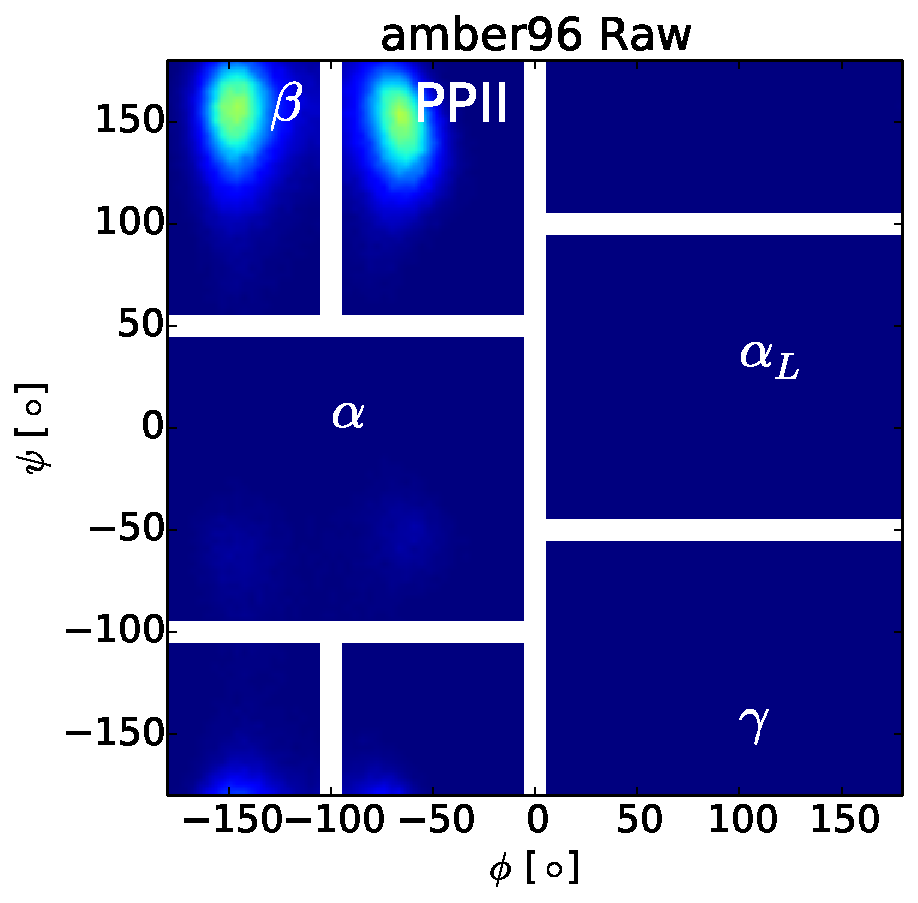
\includegraphics[width=7.05cm]{figures/ALA3_rama_amber96_raw.pdf}
}
\subfigure[]{
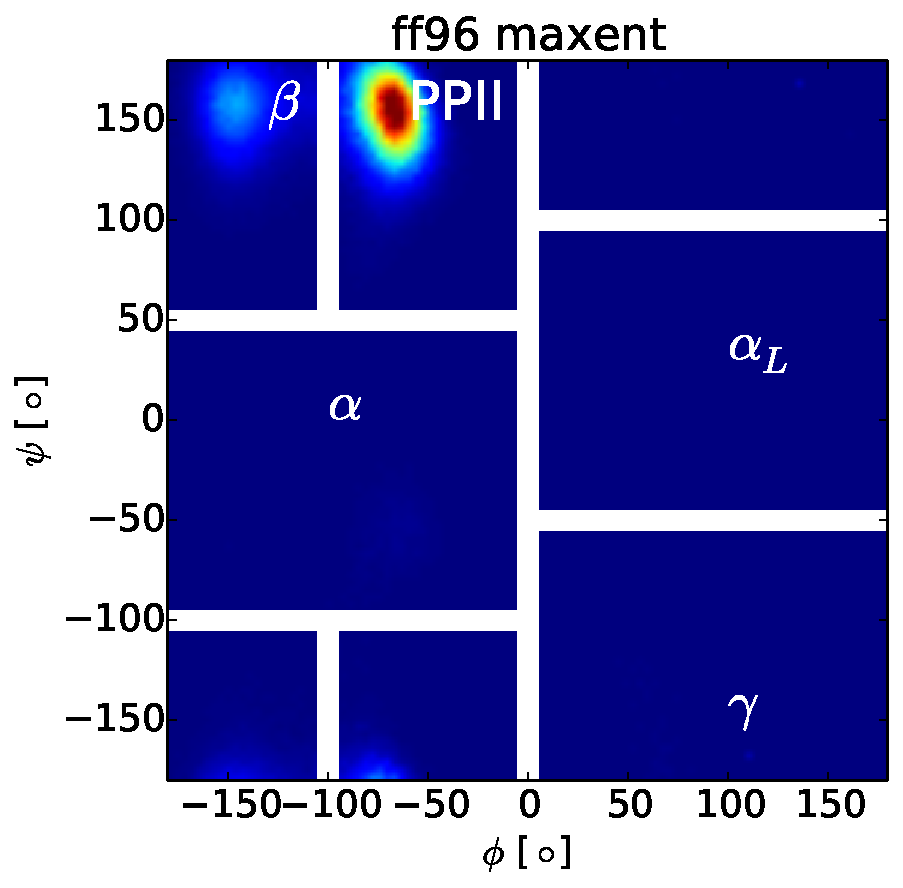
\includegraphics[width=7.05cm]{figures/ALA3_rama_amber96_maxent_belt.pdf}
}

\subfigure[]{
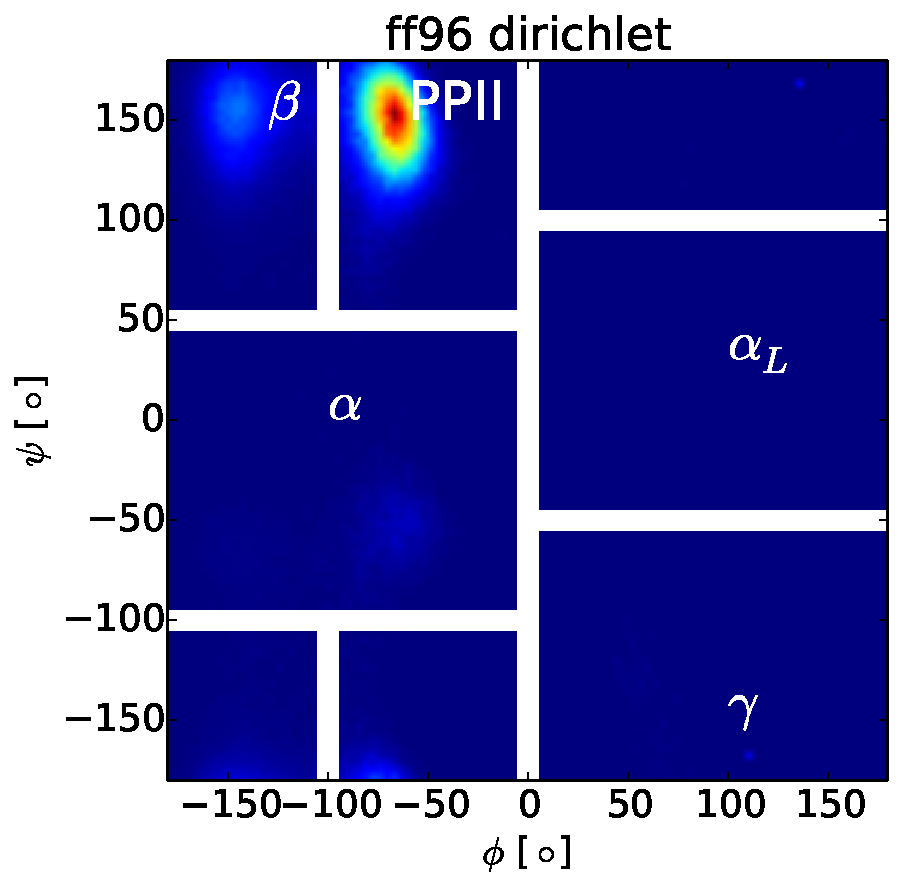
\includegraphics[width=7.05cm]{figures/ALA3_rama_amber96_dirichlet_belt.pdf}
}
\subfigure[]{
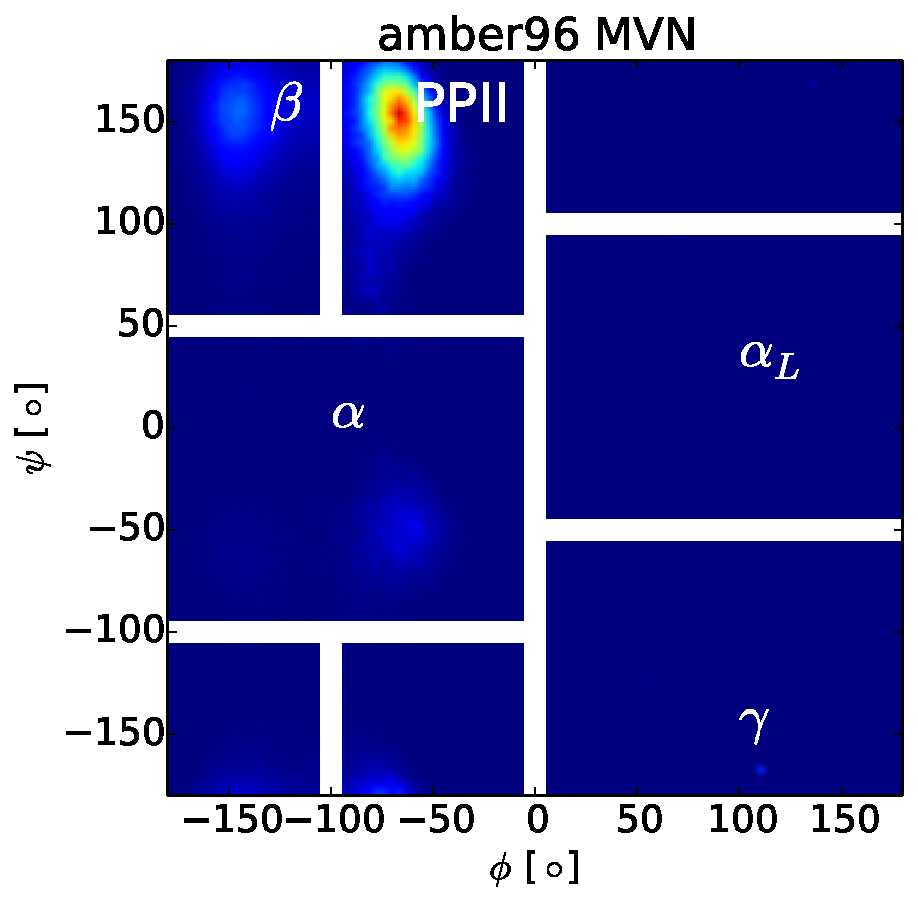
\includegraphics[width=7.05cm]{figures/ALA3_rama_amber96_MVN_belt.pdf}
}

\begin{center}
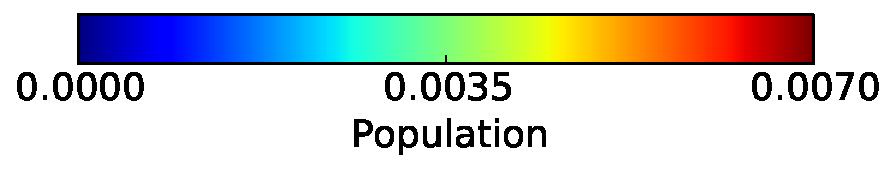
\includegraphics[width=7.05cm]{figures/ALA3_rama_colorbar.pdf}
\end{center}

\end{figure}

\newpage


\begin{figure}
\subfigure[]{
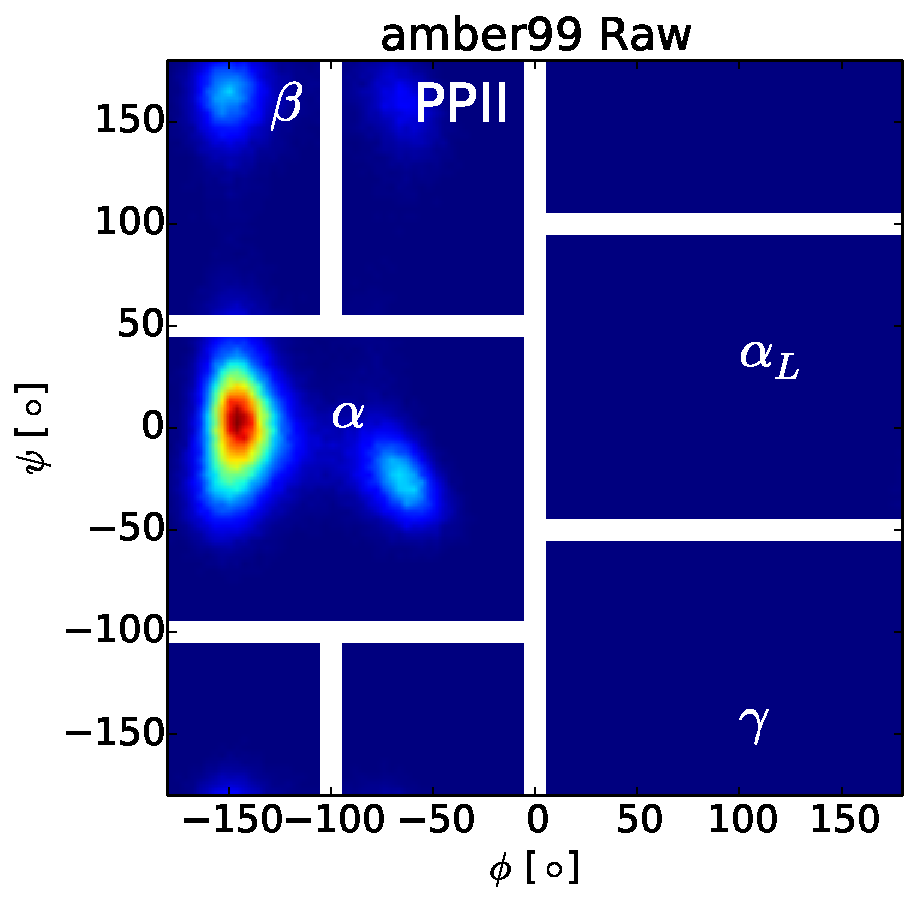
\includegraphics[width=7.05cm]{figures/ALA3_rama_amber99_raw.pdf}
}
\subfigure[]{
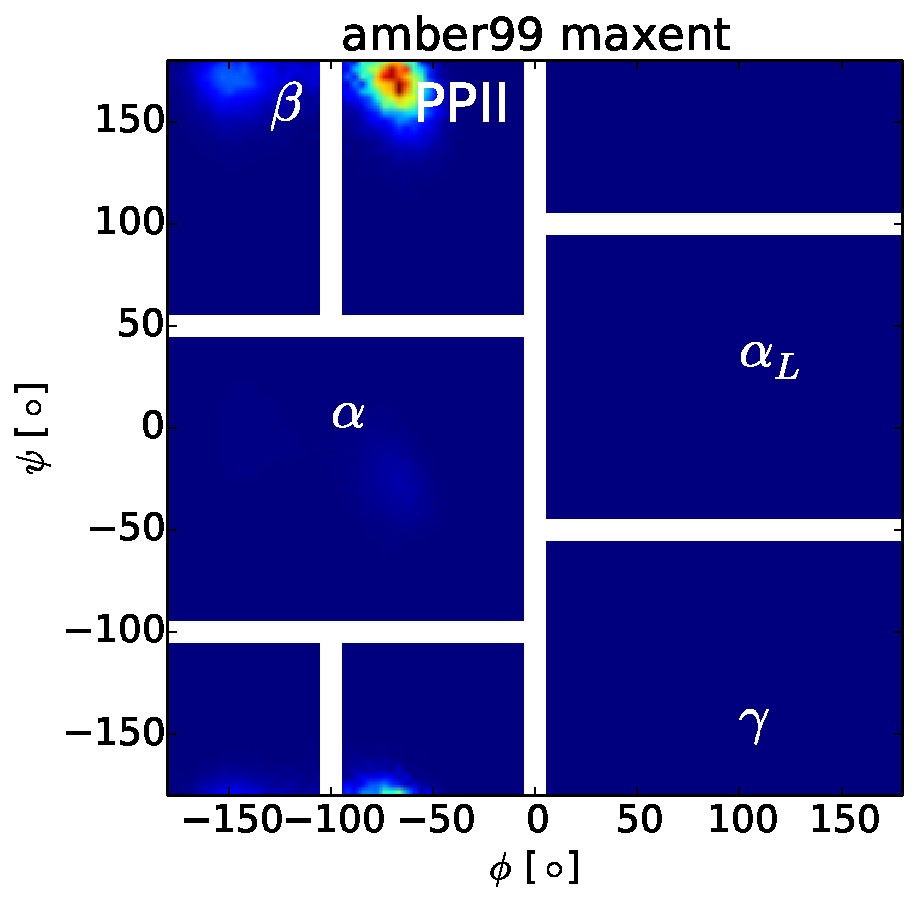
\includegraphics[width=7.05cm]{figures/ALA3_rama_amber99_maxent_belt.pdf}
}

\subfigure[]{
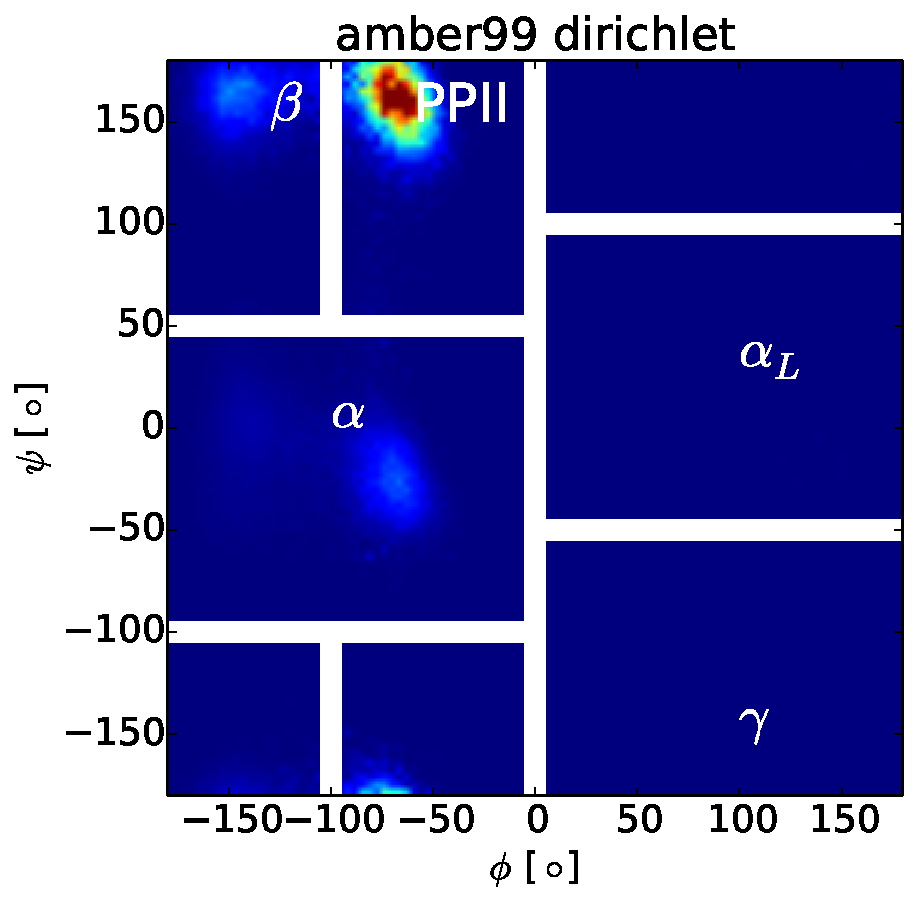
\includegraphics[width=7.05cm]{figures/ALA3_rama_amber99_dirichlet_belt.pdf}
}
\subfigure[]{
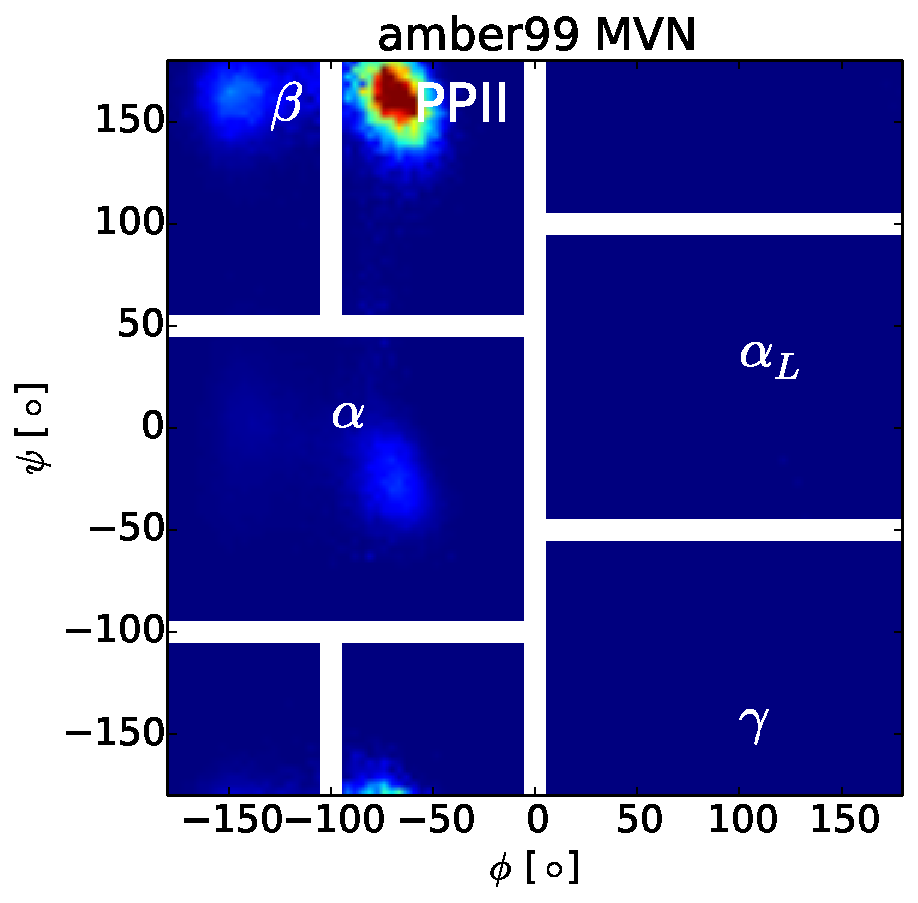
\includegraphics[width=7.05cm]{figures/ALA3_rama_amber99_MVN_belt.pdf}
}

\begin{center}
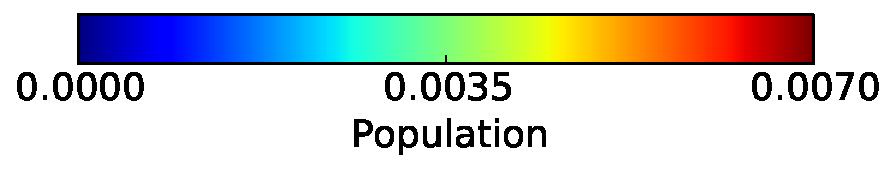
\includegraphics[width=7.05cm]{figures/ALA3_rama_colorbar.pdf}
\end{center}

\end{figure}

\newpage

\begin{figure}
\subfigure[]{
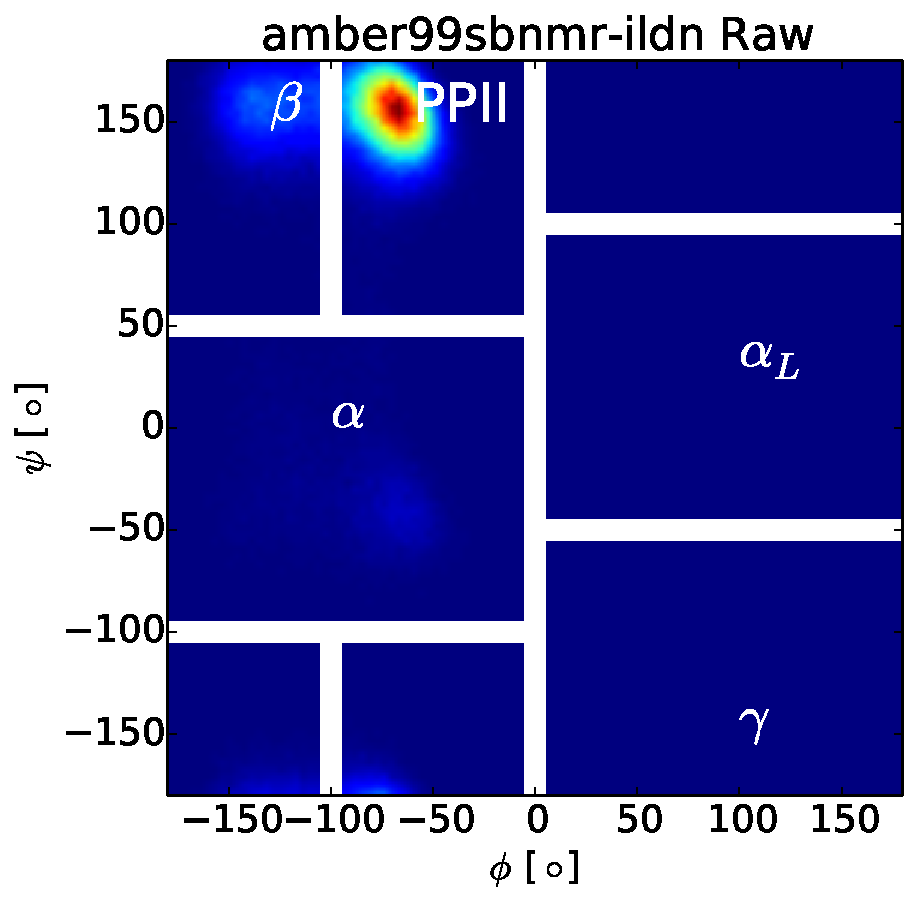
\includegraphics[width=7.05cm]{figures/ALA3_rama_amber99sbnmr-ildn_raw.pdf}
}
\subfigure[]{
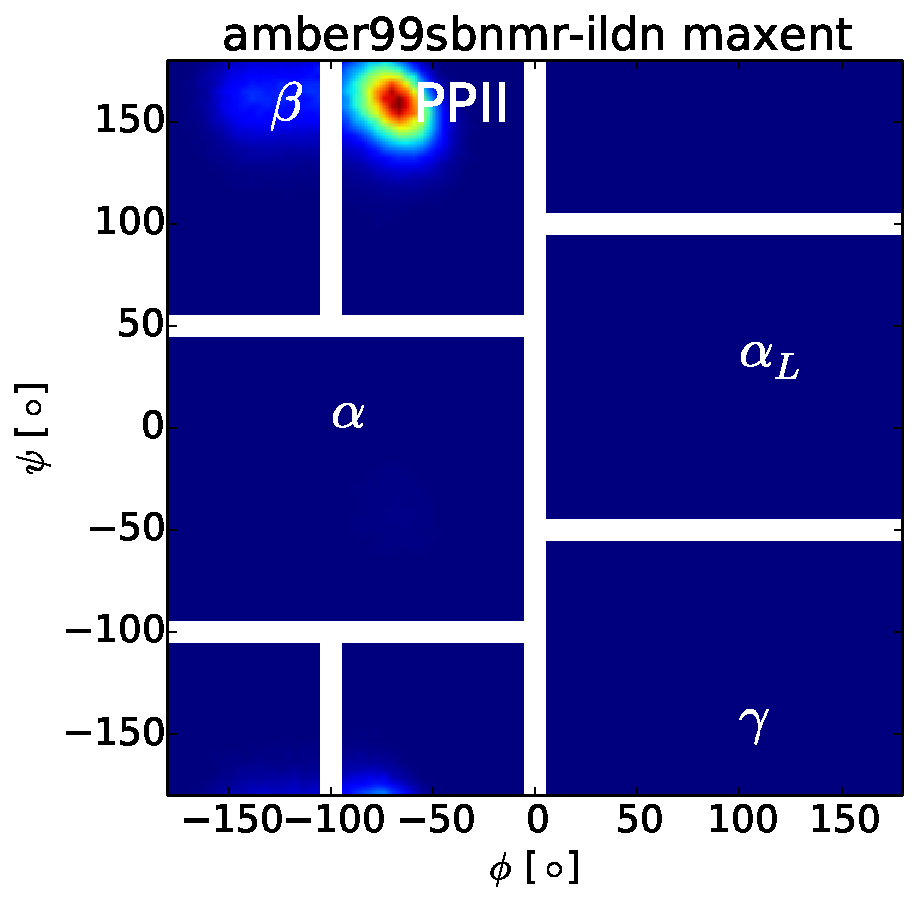
\includegraphics[width=7.05cm]{figures/ALA3_rama_amber99sbnmr-ildn_maxent_belt.pdf}
}

\subfigure[]{
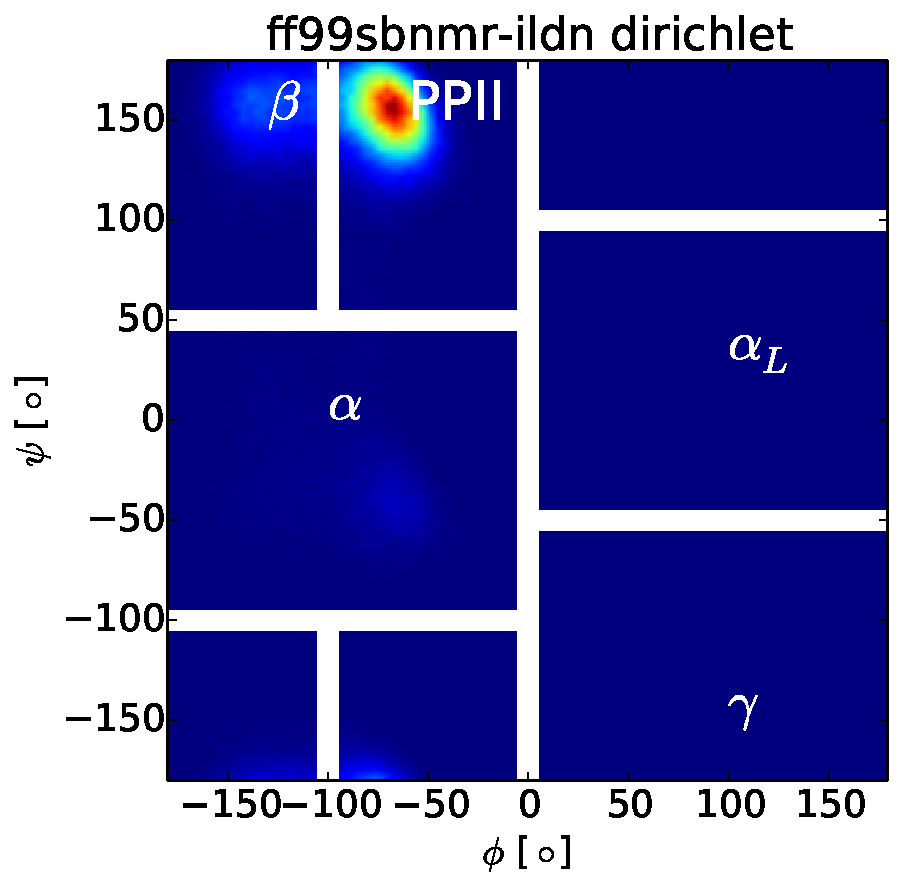
\includegraphics[width=7.05cm]{figures/ALA3_rama_amber99sbnmr-ildn_dirichlet_belt.pdf}
}
\subfigure[]{
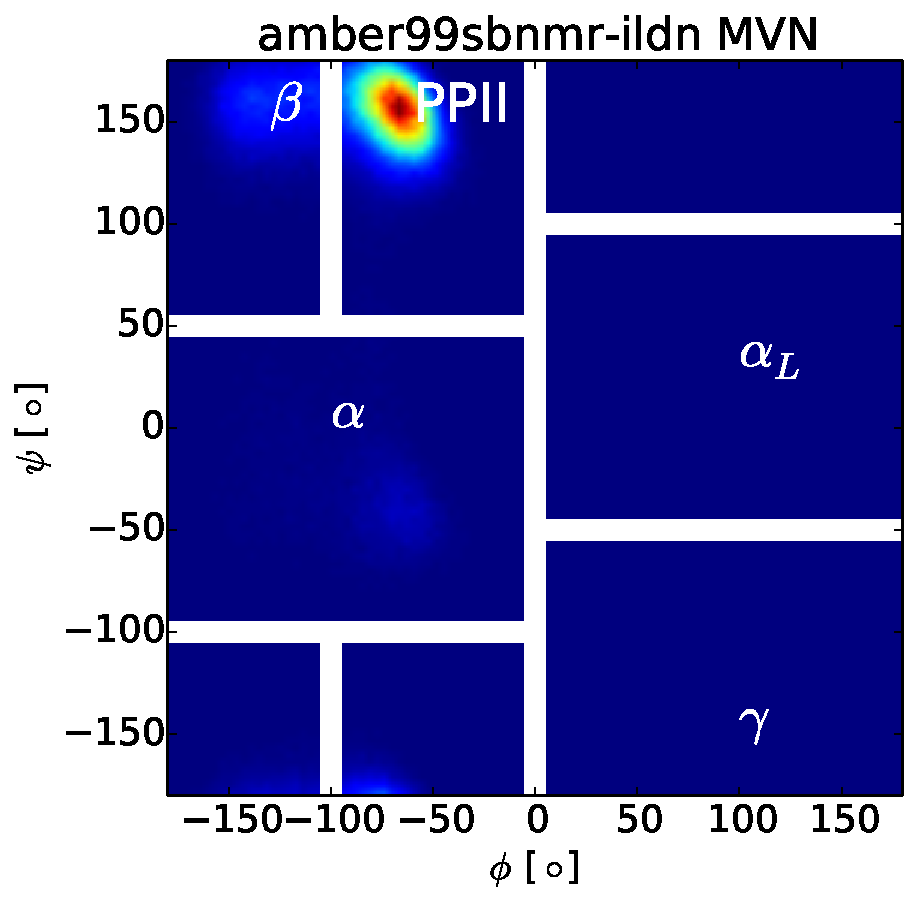
\includegraphics[width=7.05cm]{figures/ALA3_rama_amber99sbnmr-ildn_MVN_belt.pdf}
}

\begin{center}
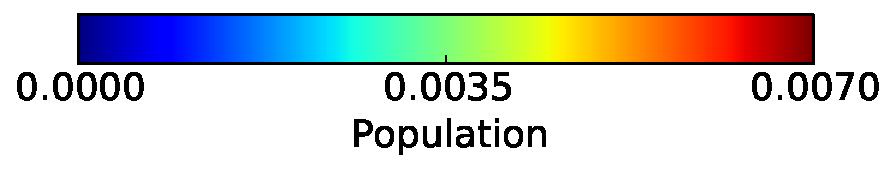
\includegraphics[width=7.05cm]{figures/ALA3_rama_colorbar.pdf}
\end{center}

\end{figure}

\newpage

\begin{figure}
\subfigure[]{
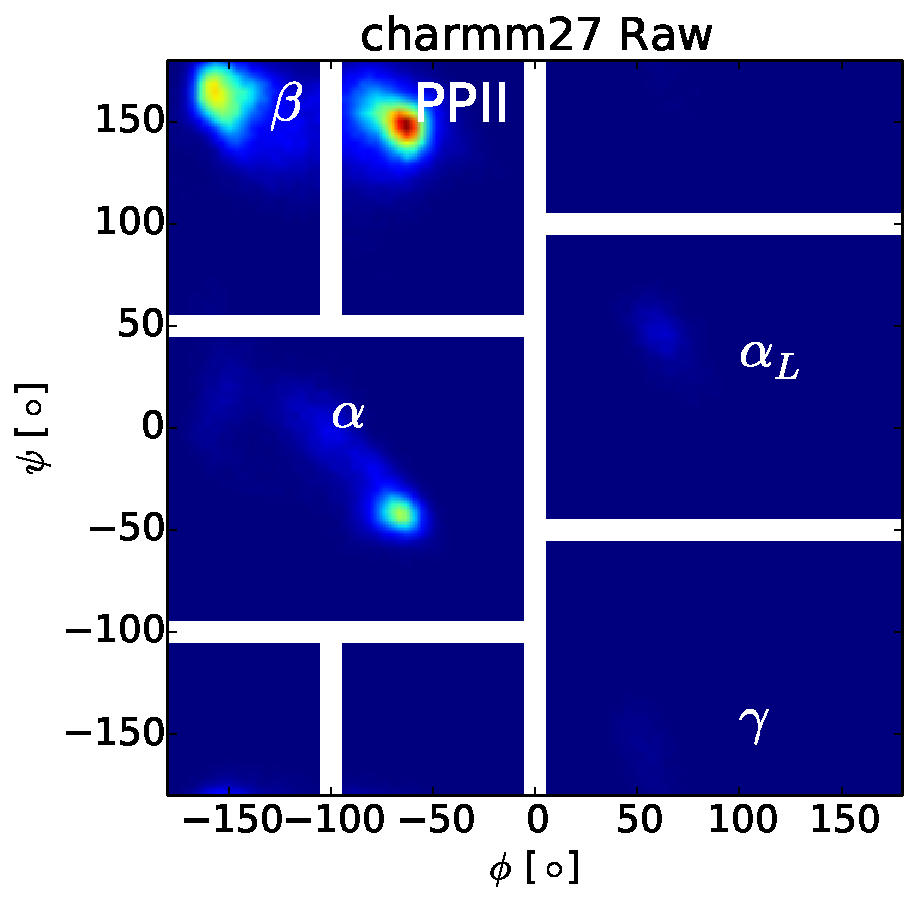
\includegraphics[width=7.05cm]{figures/ALA3_rama_charmm27_raw.pdf}
}
\subfigure[]{
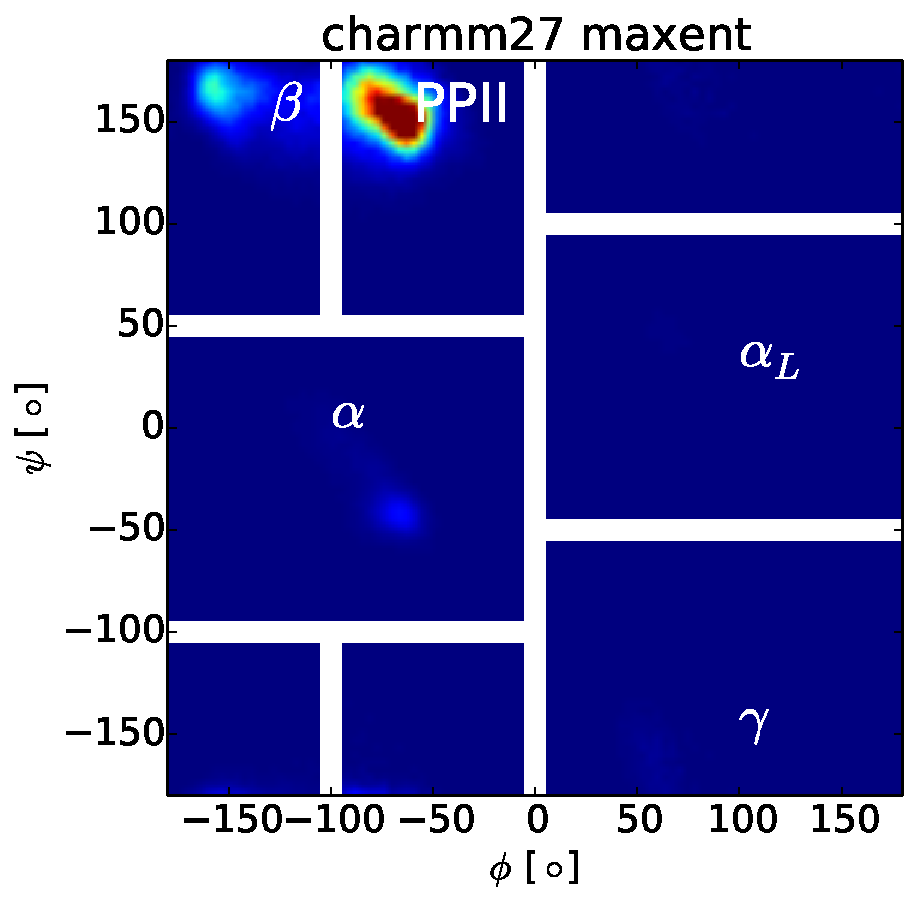
\includegraphics[width=7.05cm]{figures/ALA3_rama_charmm27_maxent_belt.pdf}
}

\subfigure[]{
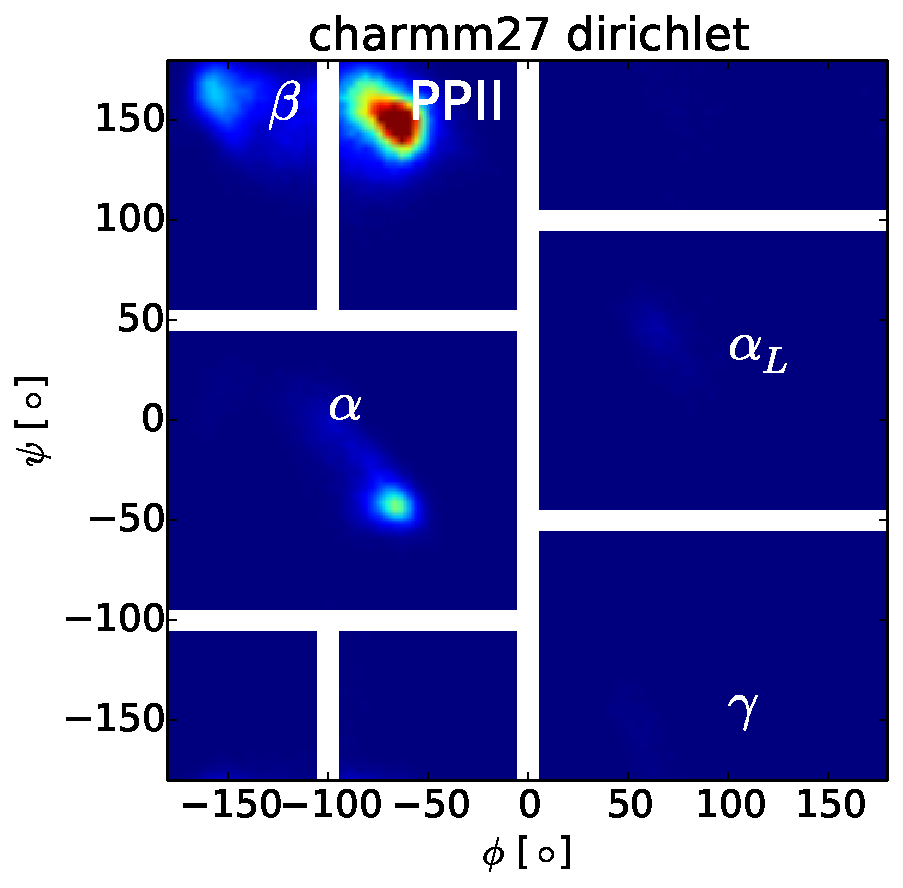
\includegraphics[width=7.05cm]{figures/ALA3_rama_charmm27_dirichlet_belt.pdf}
}
\subfigure[]{
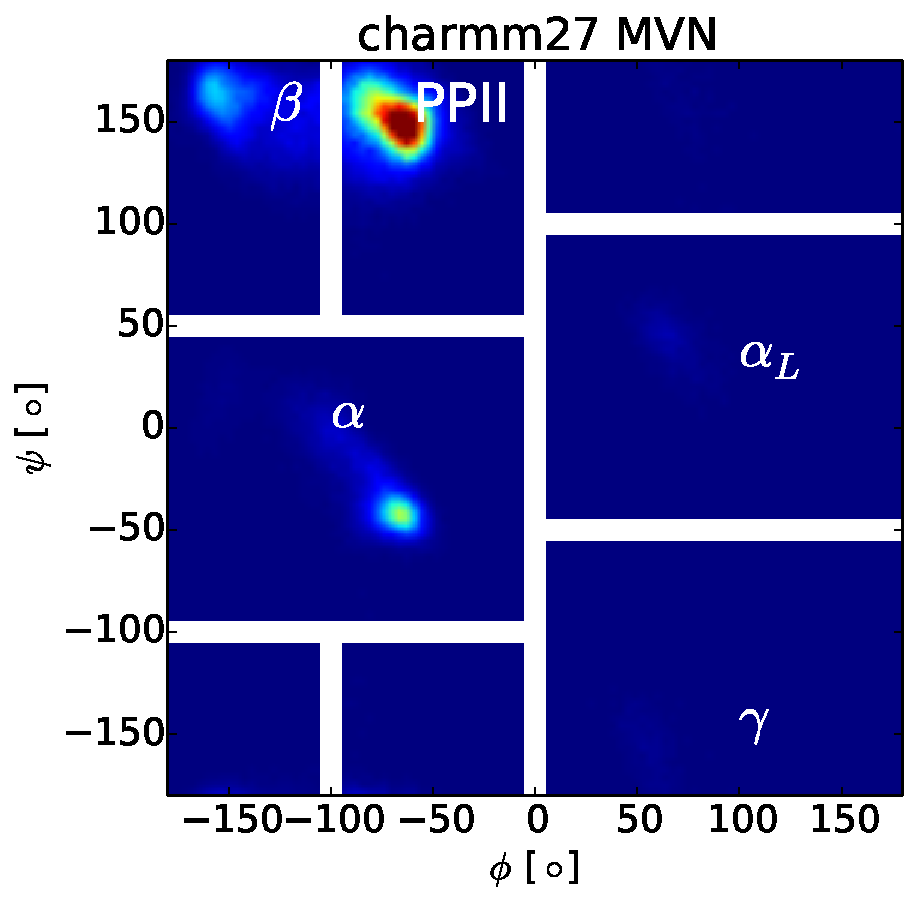
\includegraphics[width=7.05cm]{figures/ALA3_rama_charmm27_MVN_belt.pdf}
}

\begin{center}
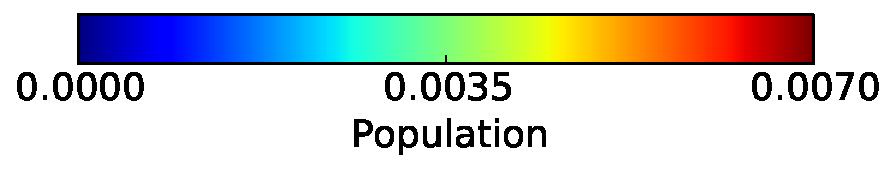
\includegraphics[width=7.05cm]{figures/ALA3_rama_colorbar.pdf}
\end{center}

\end{figure}

\newpage

\begin{figure}
\subfigure[]{
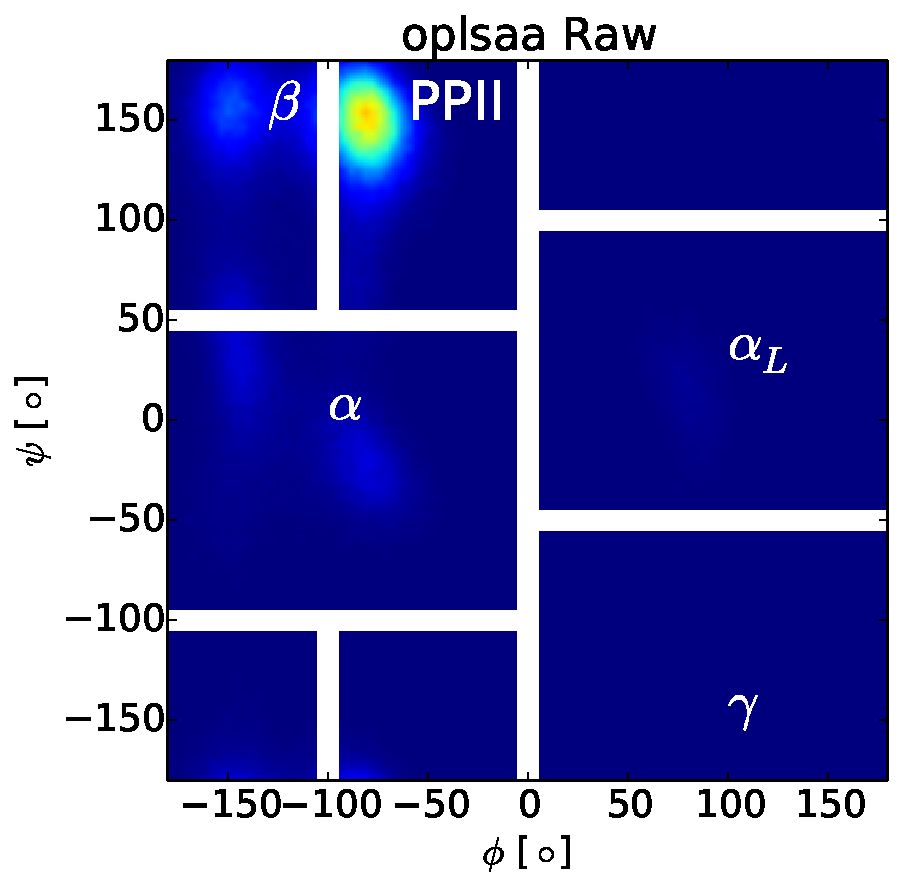
\includegraphics[width=7.05cm]{figures/ALA3_rama_oplsaa_raw.pdf}
}
\subfigure[]{
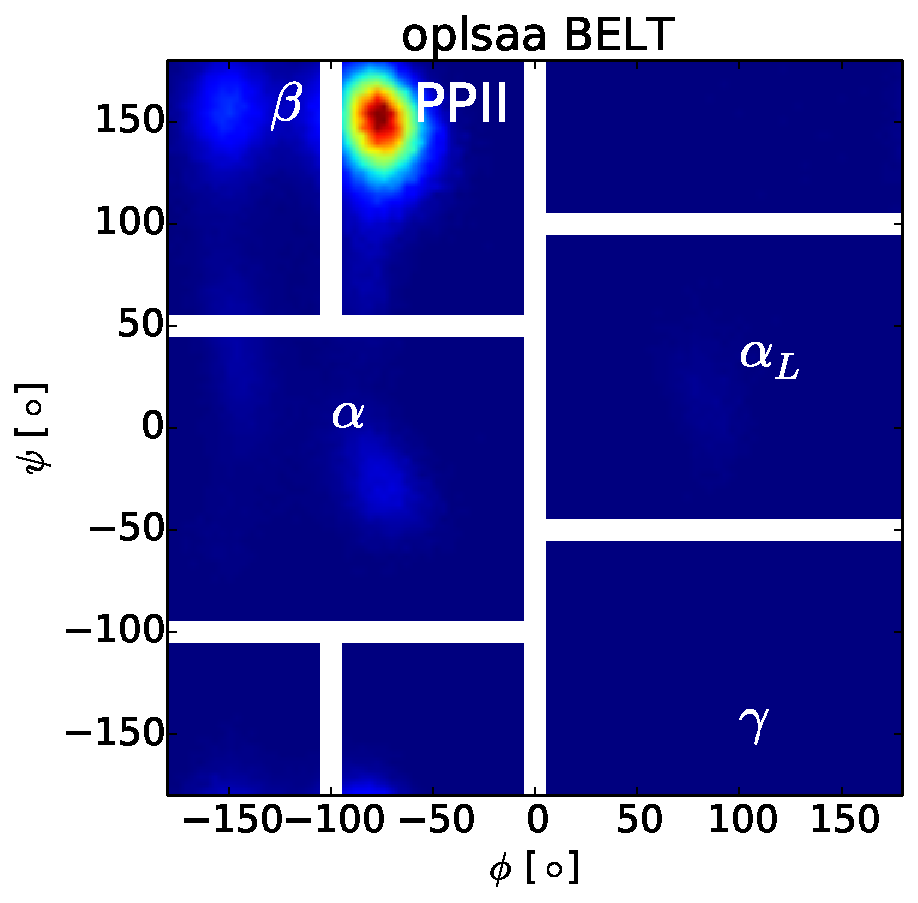
\includegraphics[width=7.05cm]{figures/ALA3_rama_oplsaa_maxent_belt.pdf}
}

\subfigure[]{
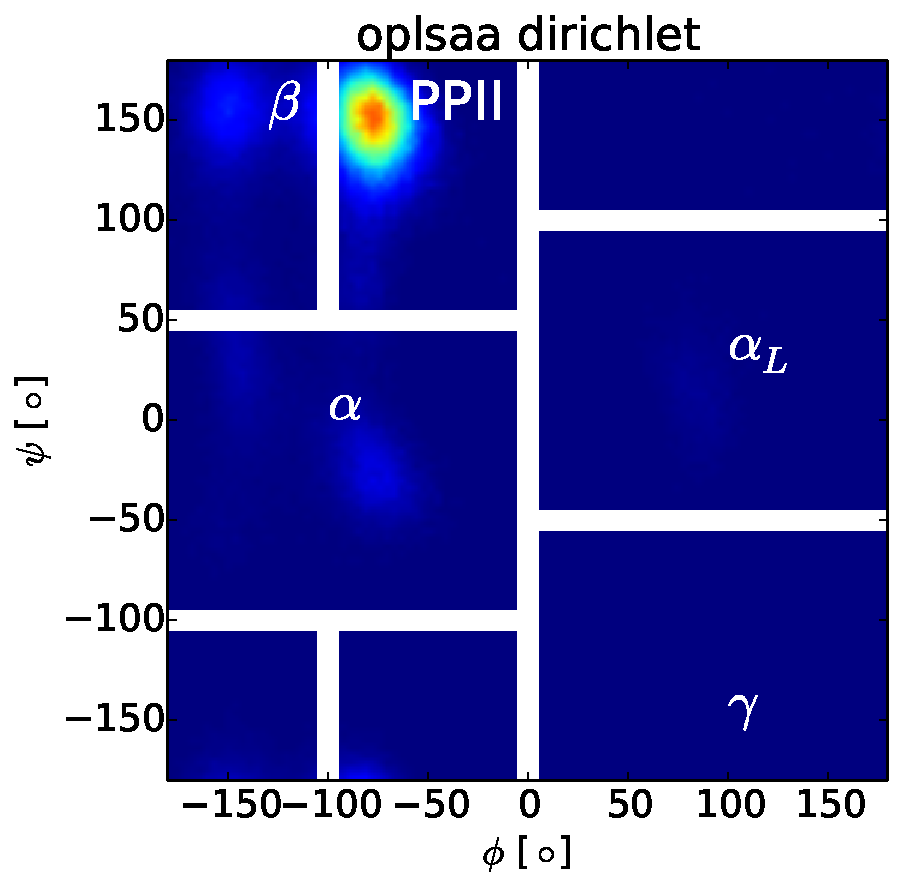
\includegraphics[width=7.05cm]{figures/ALA3_rama_oplsaa_dirichlet_belt.pdf}
}
\subfigure[]{
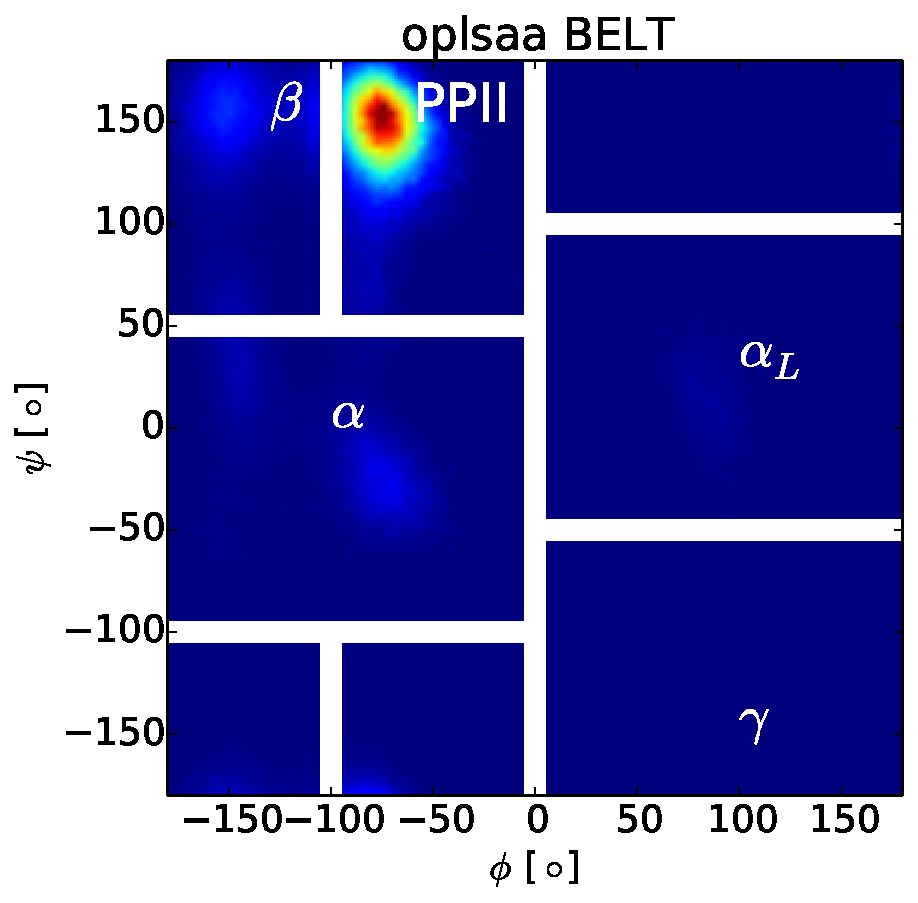
\includegraphics[width=7.05cm]{figures/ALA3_rama_oplsaa_MVN_belt.pdf}
}

\begin{center}
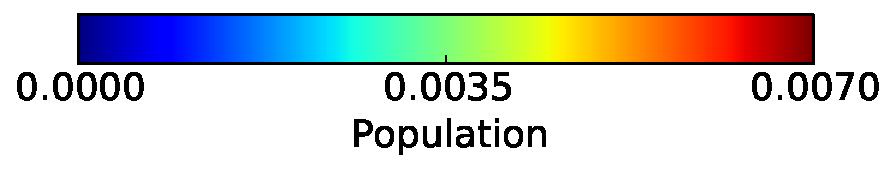
\includegraphics[width=7.05cm]{figures/ALA3_rama_colorbar.pdf}
\end{center}

\caption{
Ramachandran plots (2D histograms) of MD simulations and BELT models.  
}
\label{figure:test}


\end{figure}

\newpage


\begin{figure}
\subfigure[]{
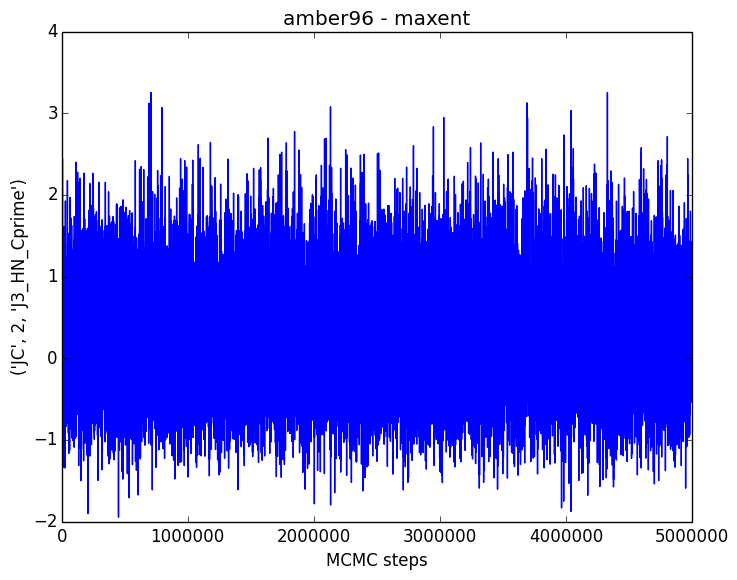
\includegraphics[width=7.5cm]{figures/maxent-amber96-MCMC_Trace.png}
}
\subfigure[]{
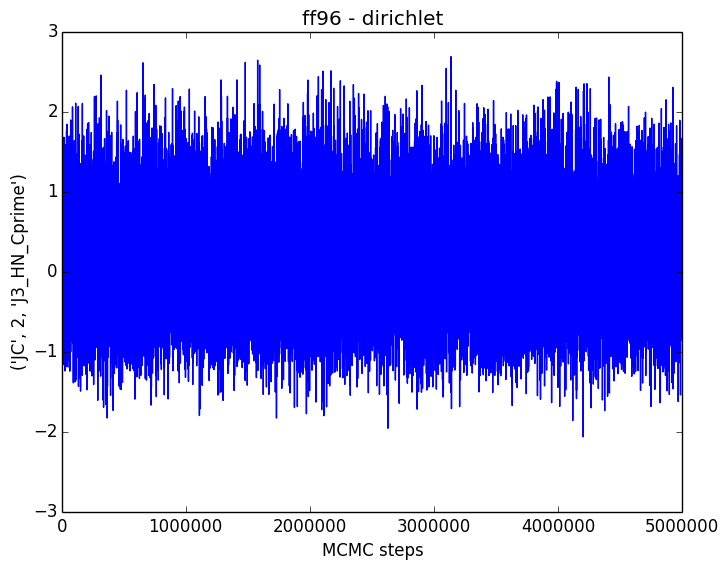
\includegraphics[width=7.5cm]{figures/dirichlet-amber96-MCMC_Trace.png}
}

\subfigure[]{
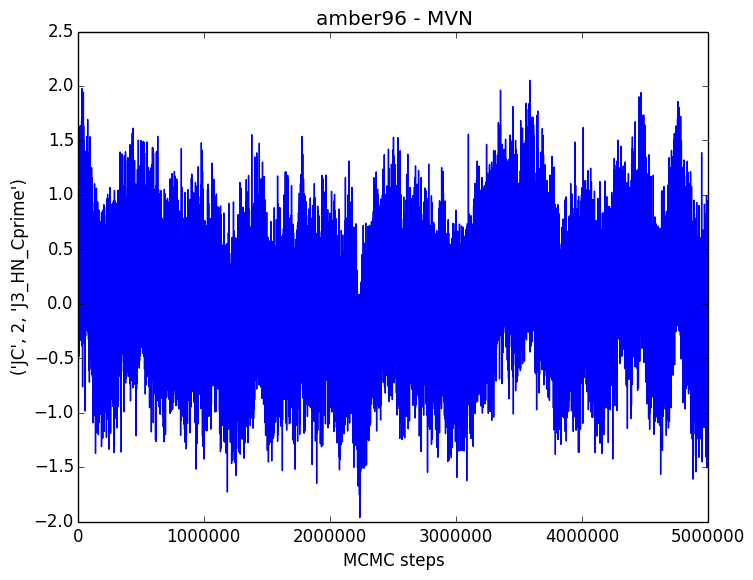
\includegraphics[width=7.5cm]{figures/MVN-amber96-MCMC_Trace.png}
}
\end{figure}

\newpage

\begin{figure}
\subfigure[]{
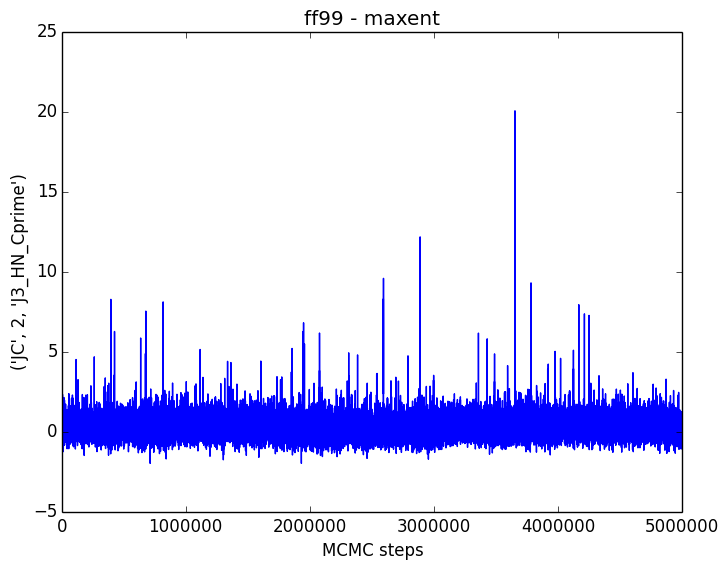
\includegraphics[width=7.5cm]{figures/maxent-amber99-MCMC_Trace.png}
}
\subfigure[]{
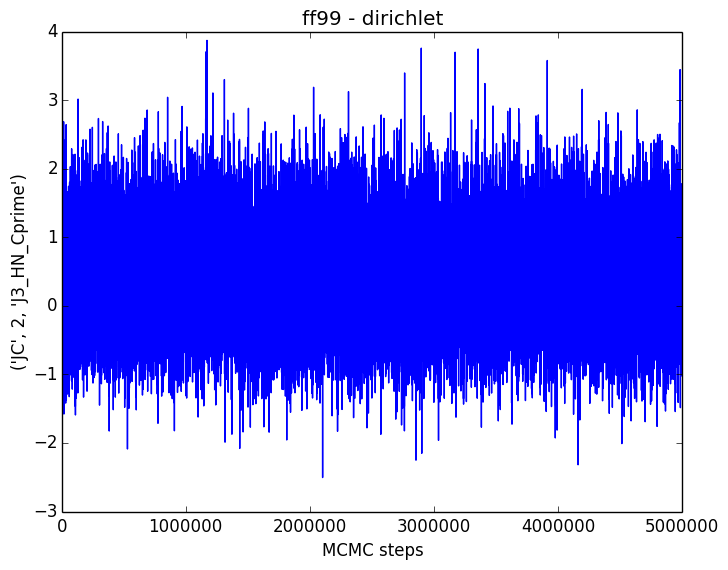
\includegraphics[width=7.5cm]{figures/dirichlet-amber99-MCMC_Trace.png}
}

\subfigure[]{
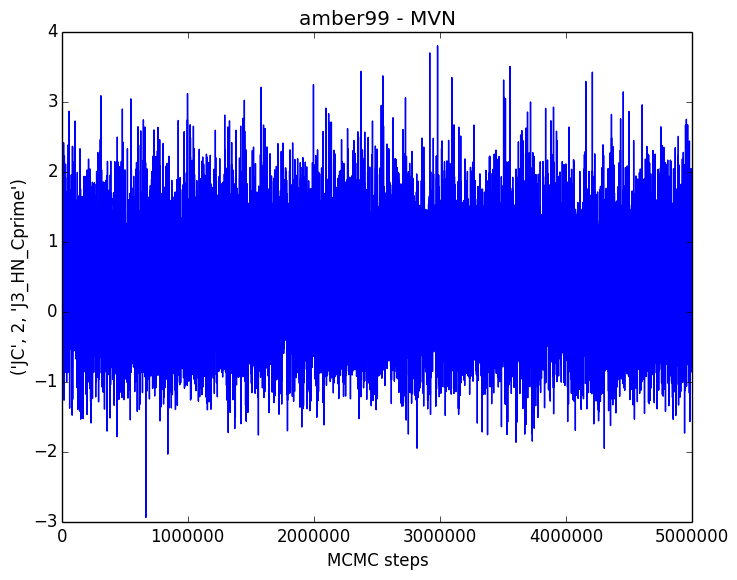
\includegraphics[width=7.5cm]{figures/MVN-amber99-MCMC_Trace.png}
}
\end{figure}

\newpage

\begin{figure}
\subfigure[]{
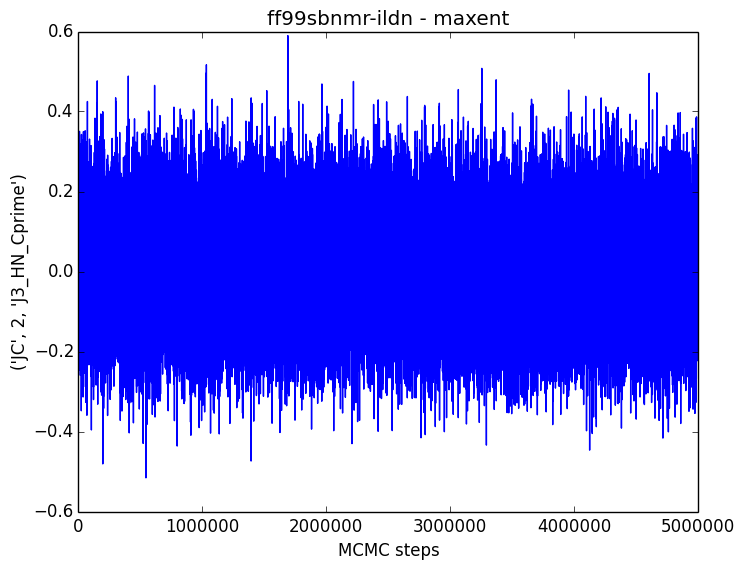
\includegraphics[width=7.5cm]{figures/maxent-amber99sbnmr-ildn-MCMC_Trace.png}
}
\subfigure[]{
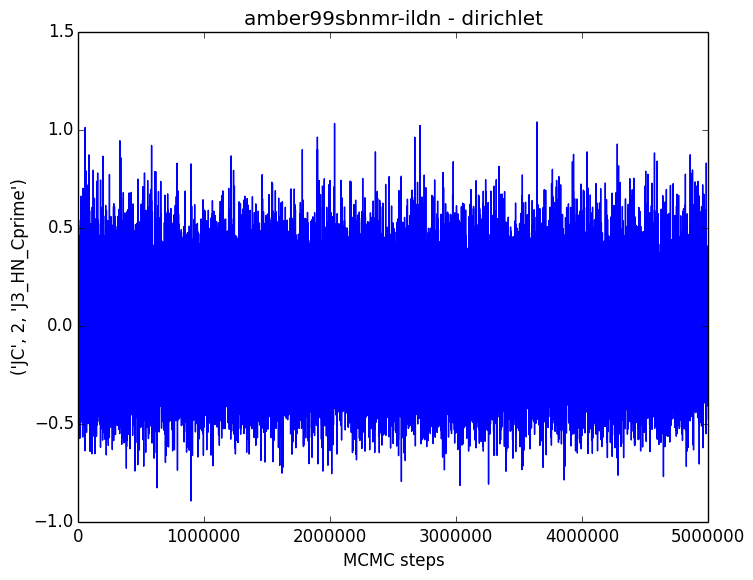
\includegraphics[width=7.5cm]{figures/dirichlet-amber99sbnmr-ildn-MCMC_Trace.png}
}

\subfigure[]{
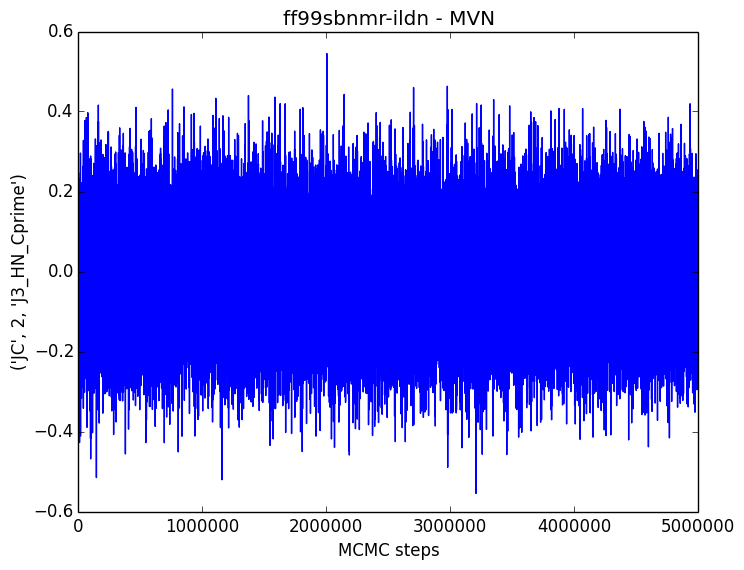
\includegraphics[width=7.5cm]{figures/MVN-amber99sbnmr-ildn-MCMC_Trace.png}
}
\end{figure}

\newpage

\begin{figure}
\subfigure[]{
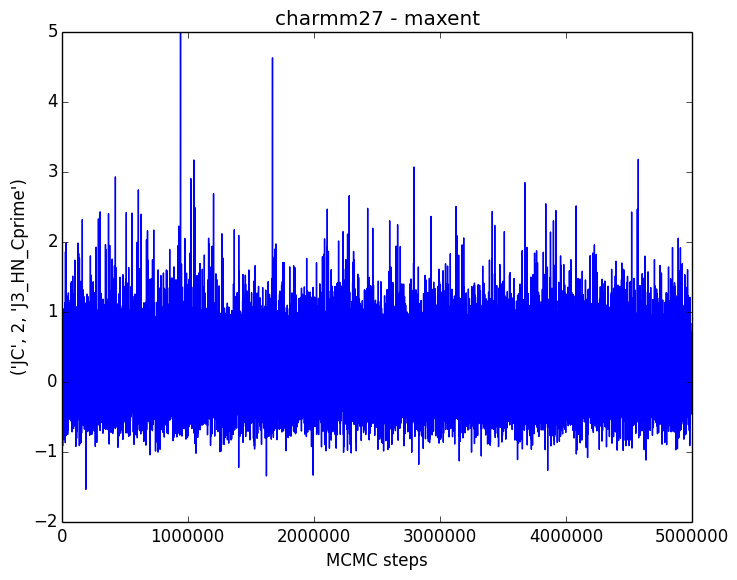
\includegraphics[width=7.5cm]{figures/maxent-charmm27-MCMC_Trace.png}
}
\subfigure[]{
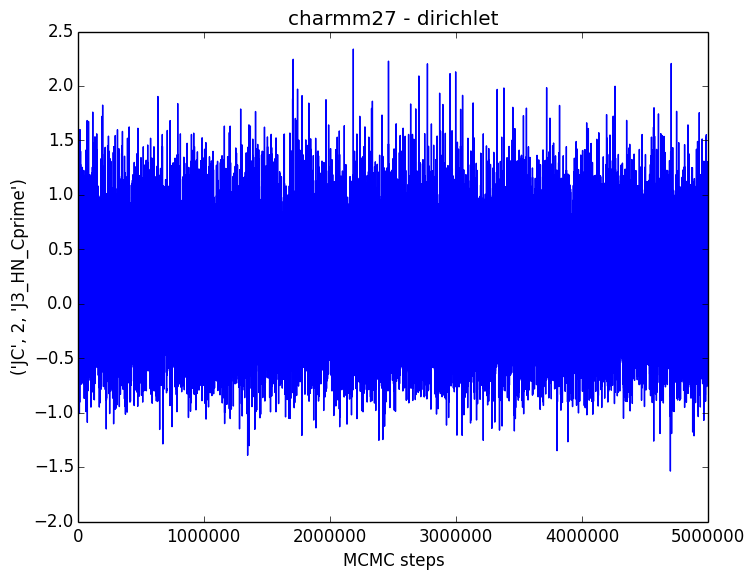
\includegraphics[width=7.5cm]{figures/dirichlet-charmm27-MCMC_Trace.png}
}

\subfigure[]{
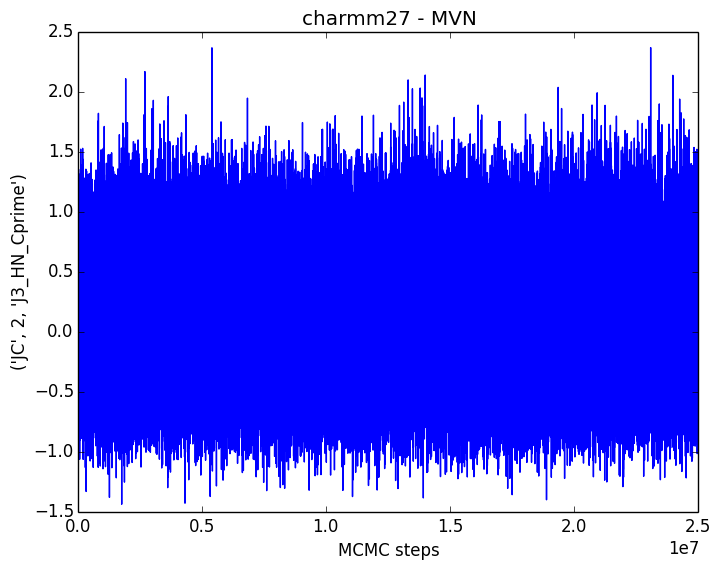
\includegraphics[width=7.5cm]{figures/MVN-charmm27-MCMC_Trace.png}
}
\end{figure}

\newpage

\begin{figure}
\subfigure[]{
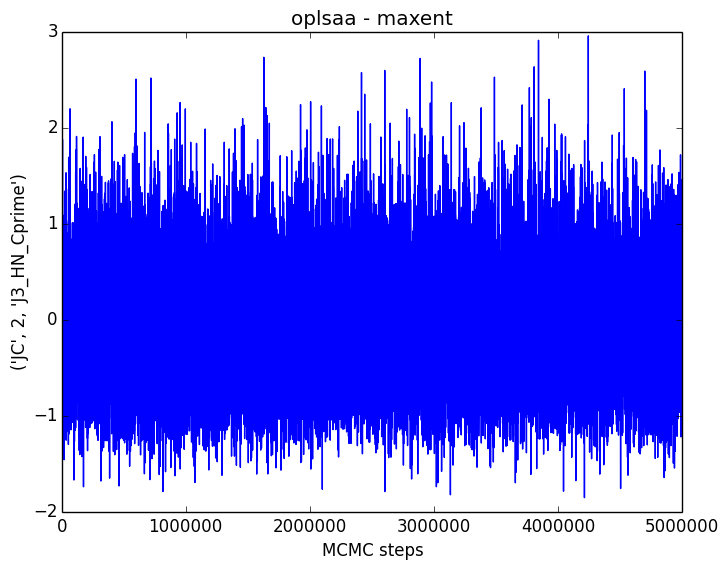
\includegraphics[width=7.5cm]{figures/maxent-oplsaa-MCMC_Trace.png}
}
\subfigure[]{
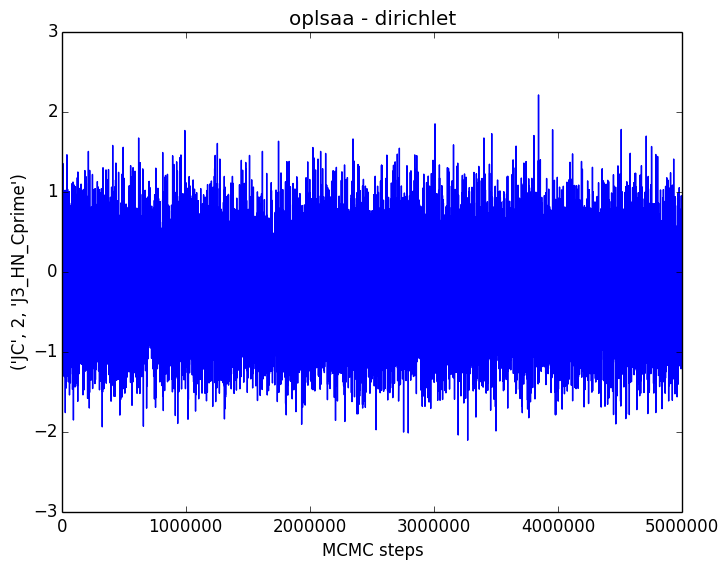
\includegraphics[width=7.5cm]{figures/dirichlet-oplsaa-MCMC_Trace.png}
}

\subfigure[]{
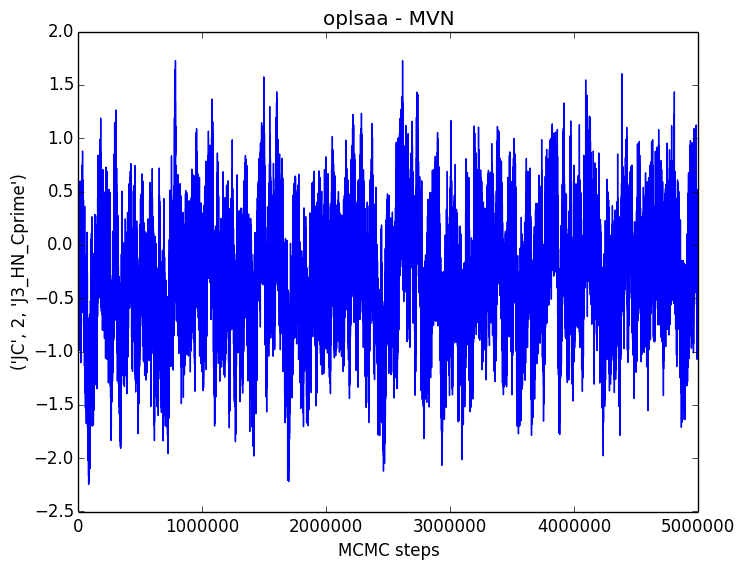
\includegraphics[width=7.5cm]{figures/MVN-oplsaa-MCMC_Trace.png}
}

\caption{
MCMC traces of first component of $\alpha$.  
}
\label{figure:MCMC}
\end{figure}

\newpage

\begin{figure}
\subfigure[]{
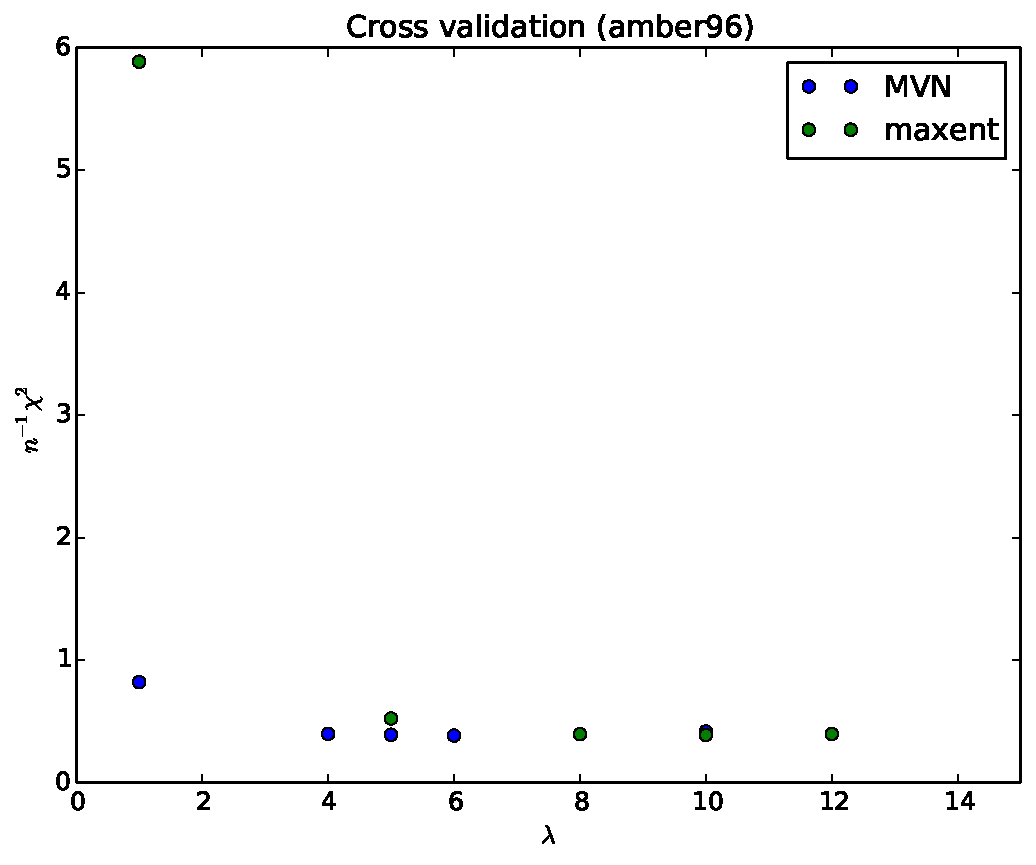
\includegraphics[width=7.5cm]{figures/cross_val_amber96.pdf}
}
\subfigure[]{
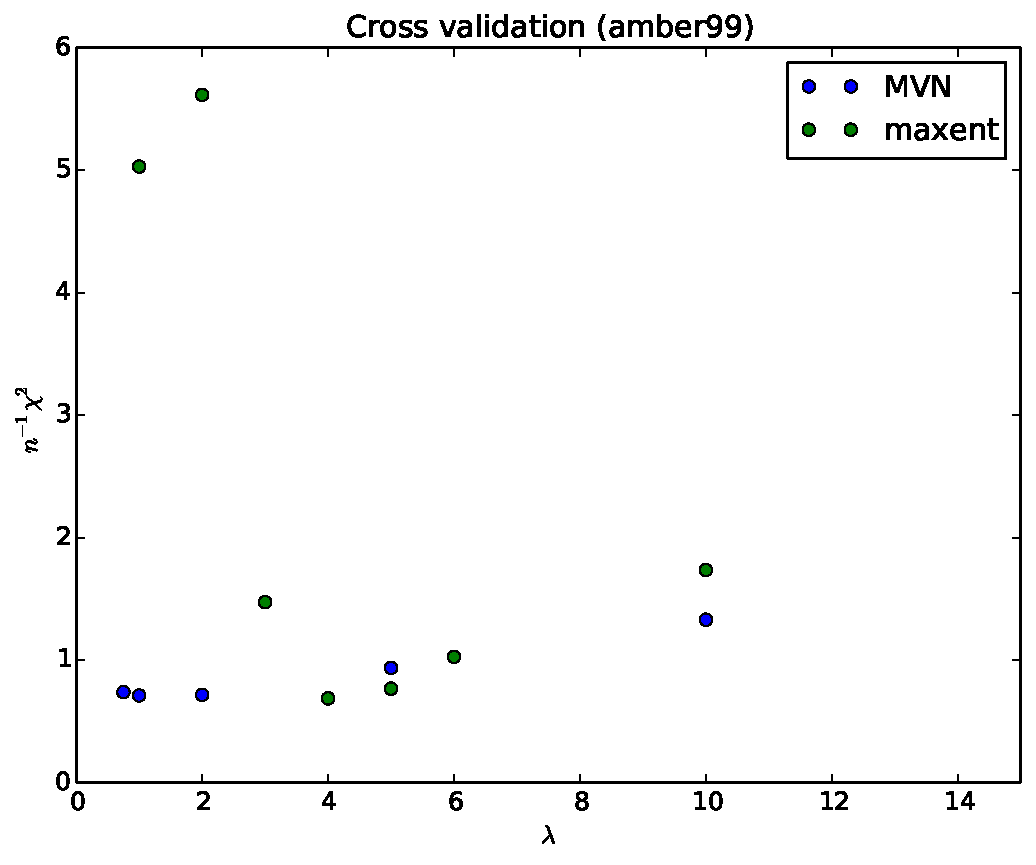
\includegraphics[width=7.5cm]{figures/cross_val_amber99.pdf}
}

\subfigure[]{
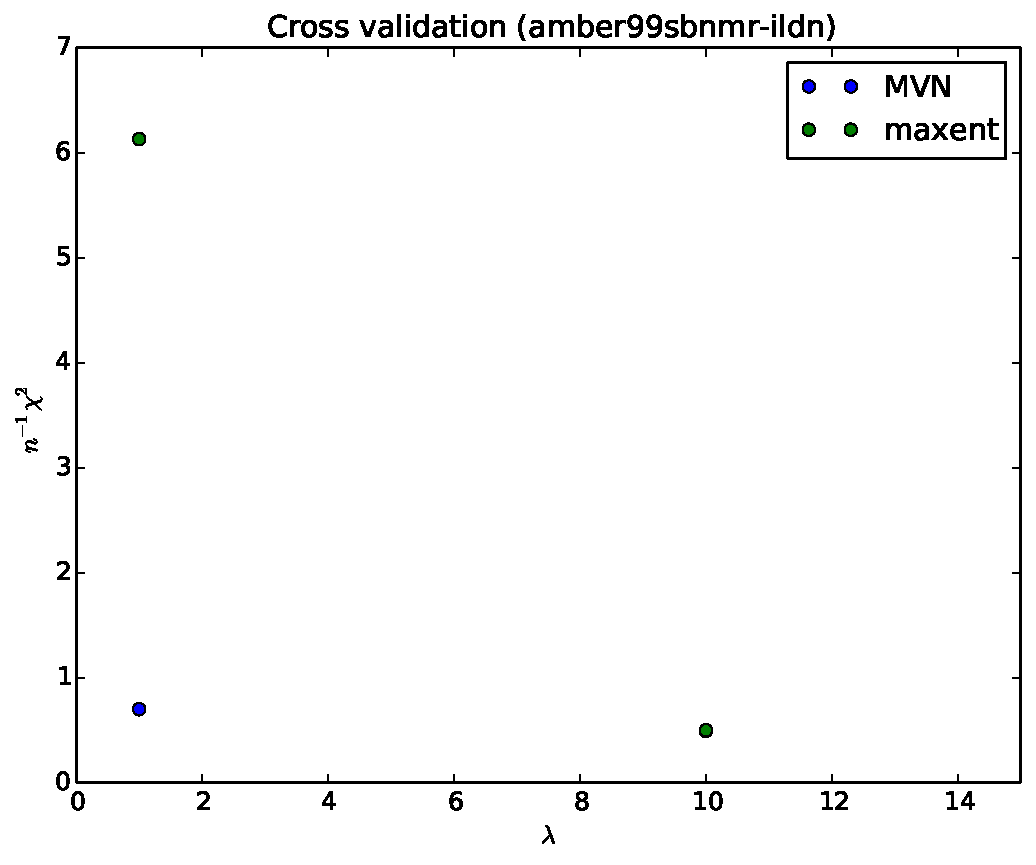
\includegraphics[width=7.5cm]{figures/cross_val_amber99sbnmr-ildn.pdf}
}

\subfigure[]{
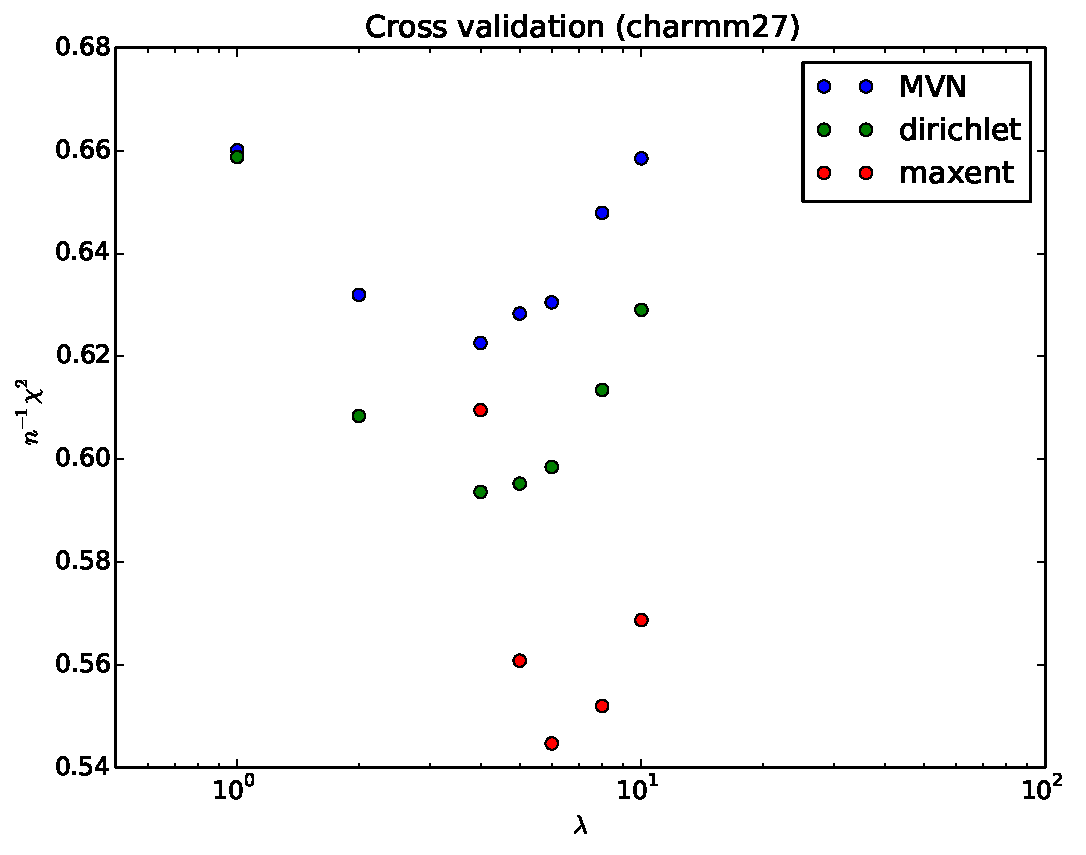
\includegraphics[width=7.5cm]{figures/cross_val_charmm27.pdf}
}
\subfigure[]{
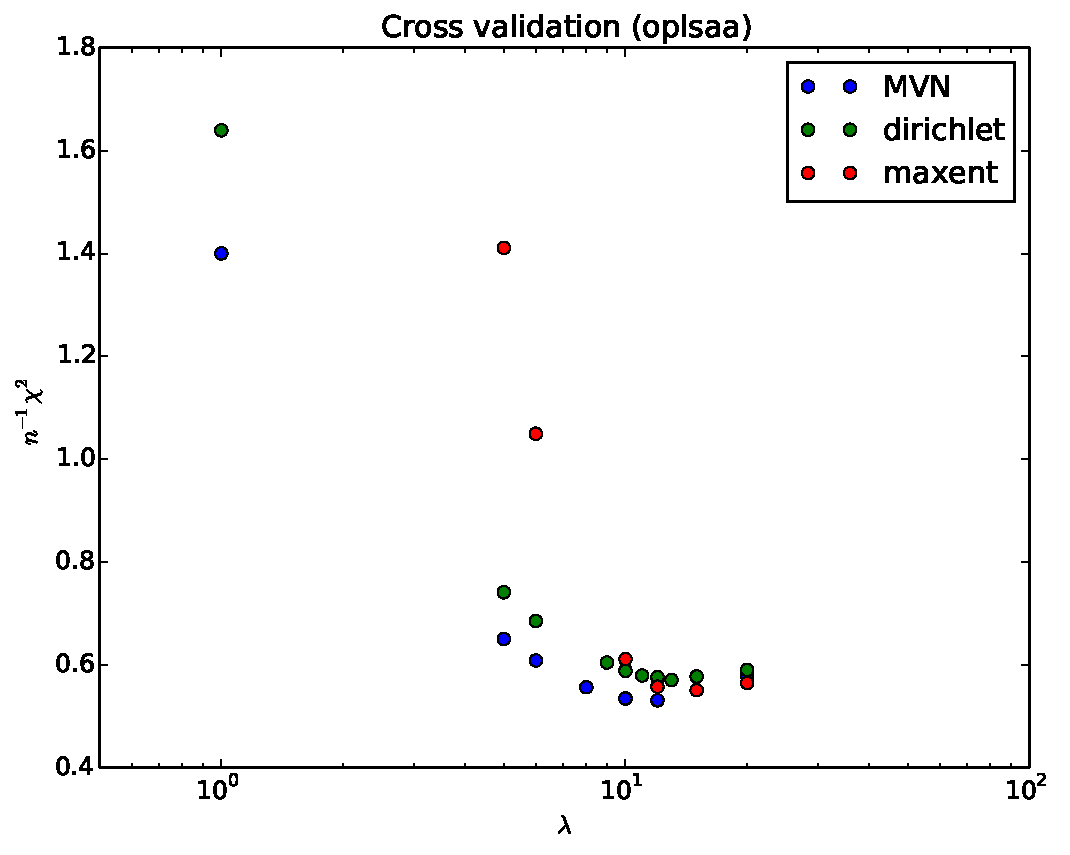
\includegraphics[width=7.5cm]{figures/cross_val_oplsaa.pdf}
}

\caption{
Cross validated reduced $\chi^2$.  Cross validation was performed using twenty-fold subsampled trajectory data to make calculations computationally tractable.  
}
\label{figure:cross_val}
\end{figure}


\clearpage

\section*{Appendix S1.  Connection between Maximum Entropy and BELT}


Bayesian Energy Landscape Tilting generalizes a recent maximum entropy formalism \cite{chodera2012} to include statistical uncertainty.  We now show the connection between the previous maximum entropy approach \cite{chodera2012} and BELT.  The previous approach minimizes an objective function $\Lambda$; it is sufficient to consider the zeros of its gradient:

$$\frac{d\Lambda}{d\alpha_k} = -\langle f_k \rangle_\alpha + F_k$$

The obvious solution, when feasible, is to set $\langle f_i(x) \rangle_\alpha = F_i$.  

In BELT, we instead sample the following log likelihood:

$$LL(\alpha) = -\sum_i \frac{1}{2\sigma_i^2}(\langle f_i\rangle _\alpha - F_i)^2 + \log P(\alpha)$$

If we assume a constant prior and maximize the likelihood, the problem becomes equivalent to setting the derivative of $LL$ to zero:

$$ \frac{dLL}{d\alpha_k} =  -\sum_i \frac{1}{\sigma_i^2} (\langle f_i\rangle _\alpha - F_i) \frac{d\langle f_i\rangle _\alpha}{d\alpha_k} = 0$$

As before, if we find a value of $\alpha$ such that $\langle f_i(x) \rangle_\alpha = F_i$, we will maximize the log likelihood.  Thus, under ideal conditions, we expect similar results using the maximum entropy approach and BELT.  


\newpage

\section*{Appendix S2.  Derivation of Reweighting}

Here we derive the population estimator used in BELT.  As in the main text, we use subscripted angle brackets to indicate ensemble averages in reweighted ensembles: $\langle h(x)\rangle _\alpha$ is the ensemble average of $h(x)$ in an ensemble that is perturbed by a biasing potential $\Delta (x;\alpha) = \sum_i \alpha_i f_i(x)$:

$$\langle h(x)\rangle _\alpha = \frac{1}{Z(\alpha)} \int h(x) dx \exp[ -U(x) - \Delta(x)]$$

$Z(\alpha)$ denotes the partition function for the $\alpha$ ensemble.  To proceed, we first note a simple Zwanzig identity that allows us to relate samples taken from different ensembles:

$$\langle h(x)\rangle _\alpha = \frac{1}{Z(\alpha)} \int h(x) dx \exp[ -U(x) - \Delta(x)] = \frac{Z(0)}{Z(\alpha)} \langle h(x) \exp[-\Delta(x;\alpha)]\rangle _0 $$

In the above expression, $\langle \rangle_0$ denotes an unperturbed ensemble (e.g. $\alpha = 0$) and $Z(0)$ is the partition function of the unbiased ensemble ($\alpha = 0$).  Now we sample from the unperturbed ensemble to statistically estimate the expectation

$$\langle h(x) \exp[-\Delta(x;\alpha)]\rangle _0 = \frac{1}{m} \sum_{j = 1}^{m} \exp [ - \Delta(x_j;\alpha)] h(x_j)$$

By letting $h(x) = 1$, we can estimate the partition function $Z(\alpha)$ up to the constant factor Z(0):

$$ \frac{Z(\alpha)}{Z(0)} = \frac{1}{m} \sum_j \exp[-\Delta(x_j;\alpha)]$$

Combining these equations, we have

$$\langle h(x)\rangle _\alpha = \sum_j h(x_j) \pi_j(\alpha)$$

where $\pi_j(\alpha)$ give estimates of the conformation weights at a particular value of $\alpha$:

$$\pi_j(\alpha) = \frac{1}{\sum_k \exp[-\Delta(x_k;\alpha)]} \exp[-\Delta(x_j;\alpha)]$$

Thus, BELT is essentially exponential averaging applied to a weighted combination of experiment-derived biasing potentials.  However, the present work has introduced two key advances.  First, the use of Markov chain Monte Carlo allows rigorous uncertainty analysis.  Second, regularization reduces the high variance previously associated with exponential averaging.  

\newpage

\section*{Appendix S3.  Alternative Error Models}

The model presented in the main text assumes independent normal deviations between measurements and the predicted ensemble.  This model is a useful approximation that leads to a straightforward $\chi^2$ likelihood.  However, in some situations, one might expect correlation between ensemble measurements.  Detecting this correlation would require additional experimental measurements.  However, it is possible to modify the $\chi^2$ likelihood to account for correlations between the predicted observables.  The net result is a modified log likelihood:

$$L L(\alpha) = \frac{1}{2} z^T P^{-1} z$$

where $P$ is the correlation matrix of the observables: $P_{ij} = Cor(f_i(x), f_j(x))$ and $z$ is the deviation between the $\alpha$ ensemble and the measurement, measured in units of the known uncertainty $\sigma_i$: $z_i = \frac{\langle f_i\rangle _\alpha - F_i}{\sigma_i}$.  Using this model will likely lead to increased estimates of uncertainties.  

Other possible error models involve modifying the assumption of normality.  A normal model penalizes models by the squared deviation from the experimental measurements.  However, expert knowledge may sometimes suggest different error models.  For example, one could imagine a model where small deviations are not penalized at all.  Such models could be inserted into the same MCMC framework with little extra effort.

\newpage

\section*{Appendix S4.  Choice of Prior}

\subsection*{Maximum Entropy (maxent) Prior}

As described in the main text, the maximum entropy prior is given by 

$$\log P(\alpha) = -\lambda \sum_j^m \pi_j(\alpha) \log \frac{\pi_j(\alpha)}{\pi_j^0}$$

Typically the reference populations are uniform; that is, $\pi_j^0 = \frac{1}{m}$.  This form of regularization has previously been used in a likelihood formalism to model SAXS ensembles \cite{rozycki2011saxs}.  

\subsection*{Dirichlet Prior}

We also consider the Dirichlet prior.  Dirichlet priors are commonly used as conjugate priors to multinomial random variables--that is, when dealing with counts and probabilities of categorical data.  The Dirichlet distribution is nonzero on the unit simplex and has the following functional form:

$$f(\pi;s) = \frac{1}{B(s)} \prod_j \pi_j^{s_j - 1}$$

The Dirichlet prior is an obvious choice for BELT, because the object of interest is the probability distribution on conformations.  However, in BELT, we must restrict the distribution to the subset of probability distributions that can be achieved via reweighting.  Thus, instead of $x_j$, we have $\pi_j(\alpha)$:

$$f(\alpha;s) = \frac{1}{B(s)} \prod_j \pi_j(\alpha)^{s_j - 1}$$

For our MCMC calculations, we work with the $log$ probability:

$$\log f(\alpha;s) = -\log(B(s)) + \sum_j (s_j - 1) \log \pi_j(\alpha)$$

Note that the constant term is unimportant, as MCMC relies on the difference in $log$ probabilities:

$$\log f(\alpha;s) \approx \sum_j (s_j - 1) \log \pi_j(\alpha)$$

In practice, the maxent prior has a large number of hyperparameters--the pseudocounts $s_i$ on each conformation.  To avoid the need for many hyperparameters, we assume that 

$$s_j - 1 = \lambda \pi_j^0$$

Thus, we assume that the pseudocounts are proportional to the raw MD simulation populations, which for constant temperature MD should be a uniform distribution.  For practical implementation in an MCMC sampler, we can drop terms that do not depend on $\alpha$, which leads to the following:

$$\log f(\pi;s) =  \lambda \sum_j \pi_j^0 \log \pi_j(\alpha)$$

Note that this can be rearranged into the following form, which better illuminates the connection between the maxent and Dirichlet priors:

$$\log P(\alpha) = -\lambda \sum_j \pi_j^0 \log \frac{\pi_j^0}{\pi_j(\alpha)}$$

Notice that this functional form is quite similar to the maxent prior that we previously discussed.  The difference between the maxent and Dirichlet priors can be explained in terms of the relative entropy between two distributions $P$ and $Q$.  The relative entropy is given by

$$D_{KL}(P||Q) = \sum_i P_i \log \frac{P_i}{Q_i}$$

The relative entropy is not a symmetric relationship--that is, $D_{KL}(P||Q) \ne D_{KL}(Q||P)$.  The maxent and Dirichlet priors are simply the relative entropy between $\pi(\alpha)$ and a reference distribution $\pi^0$, calculated in either direction.    For equilibrium molecular dynamics, the reference distribution is simply uniform ($\frac{1}{m}$).


\subsection*{Multivariate Normal (MVN) Prior}

In the MVN prior, $\alpha \sim N(\mu,\Sigma)$.  We let $\mu = 0$ to center the MVN around $\alpha = 0$.  This places the highest prior density on the raw simulation and allows regularization of $\alpha$.  To pick $\Sigma$, we note that the simple choice of $\Sigma_{ij} = \delta_{ij}$ leads to a prior that depends on the units of $\alpha$; this dependence on the unit system is undesirable.  However, if we choose $\Sigma_{ij} = \lambda Cov(f_i(x), f_j(x))$, the units of $\alpha_i$ and $f_i(x)$ cancel out in the MVN likelihood, leaving a result that is unit-invariant.  We have also introduced a scaling factor $\lambda$ to tune the amount of regularization.


\subsection*{Jeffrey's Prior}

Another choice of prior would be to use the Jeffrey's prior, which is uninformative and invariant under reparameterization.  We found Jeffrey's prior to be less desirable, however, because it does not necessarily place the prior maximum at $\alpha = 0$--thus, Jeffrey's prior was unable to provide regularization.  Regardless, we derive Jeffrey's prior below.

\subsection*{Derivation of Jeffrey's Prior}

This section derives the Jeffrey's prior for the BELT likelihood.  We do not recommend the use of this prior, as it is expensive to compute and unable to provide regularization.  This section can be skipped by most readers; we include it only for completeness.

Jeffrey's prior dictates that 

$$P(\alpha) \propto \det(I(\alpha))^\frac{1}{2}$$

The Fisher information matrix, $I(\alpha)$, is given by

$$I_{ab}(\alpha) = E_\alpha(\frac{d\log P(F|\alpha)}{d\alpha_{a}}\frac{d\log P(F|\alpha)}{d\alpha_{b}})$$

First, we examine the log likelihood (dropping terms independent of $\alpha$) and calculate its derivative:

$$LL = \log P(F|\alpha) = - \frac{1}{2}\sum_i (\frac{F_i - \langle F_i\rangle_\alpha}{\sigma_i})^2$$

$$\frac{d(LL)}{d\alpha_a} = \sum_i \frac{1}{\sigma_i}(F_i - \langle F_i \rangle_\alpha) \frac{d\langle F_i \rangle_\alpha}{d\alpha_a}$$

When we insert this equation into the expectation, only $(F_i - \langle F_i \rangle_\alpha)$ depends on $F_i$.  The remaining terms can be pulled outside the expectation:

$$I_{ab} = \sum_{ij} \frac{d\langle F_i \rangle_\alpha}{d\alpha_a} \frac{d\langle F_j \rangle_\alpha}{d\alpha_b} E(\frac{1}{\sigma_i \sigma_j}(F_i - \langle F_i \rangle_\alpha)(F_j - \langle F_j \rangle_\alpha))$$

Because the conditional likelihood is a diagonal multivariate normal, the expectation is simply $\delta_{ij}$, leading to 

$$I_{ab} = \sum_{i} \frac{d\langle F_i \rangle_\alpha}{d\alpha_a} \frac{d\langle F_i \rangle_\alpha}{d\alpha_b} $$

Now, we know that 

$$\frac{d\langle F_i \rangle_\alpha}{d\alpha_a} = \sum_k f_{ak} \frac{d\pi_k}{d\alpha_a}$$

where $f_{ak} = f_a(x_k)$.  Similarly, we can show that

$$\frac{d\pi_k}{d\alpha_a} = \pi_k (\langle F_a \rangle_{\alpha} - f_{ak})$$


Putting all this together, we can show that

$$I = S^T S$$

Where 

$$S_{ia} = \sum_k \pi_k (<F_a>_\alpha - f_{ka}) f_{ki}$$

\newpage

\section*{Appendix S5.  Determining Prior Strength Via Cross-Validation}

Each prior in this work contains a single free parameter, $\lambda$, which controls the level of regularization.  At least two different approaches can help select an appropriate value of $\lambda$:

\begin{enumerate}
 \item Cross validation on simulation data (used in main text)
 \item Cross validation on experimental data
\end{enumerate}

\subsection*{Cross validation on simulation data}

We first discuss cross-validating on the simulation data.  The underlying idea is that too little regularization ($\lambda = 0$) leads to models that overfit the available simulation data and generalize poorly--that is, repeating or extending the MD simulations would lead to a different result.  At the other extreme, underfit models ($\lambda = \infty$) will simply report the unbiased simulations, leading to poor agreement with experiment.  To perform this form of cross-validation, first separate the simulation data into several independent subsets.  Mark one subset as the ``test'' set and fit the model on the remaining data (the ``training'' set).  The $\chi^2$ score is evaluated on the test data.  We then repeat the process, letting the test set be equal to each of the other subsets.  The final $\chi^2$ square is averaged over each of these iterations.  The value of $\lambda$ is chosen to minimize the test set error.

When using MD to generate conformations, you must perform cross-validation using uncorrelated subsets of the data.  This precludes the typical standard cross-validation approach that uses randomly selected subsets of your data--randomly selected folds will be tainted by correlation between the folds.  As a thought experiment, suppose you do cross validation by dividing your trajectory into even and odd frames.  Because of time-correlation in the data, the even and odd subsets will essentially contain the same information--ruining the cross-validation.  To avoid these perilous correlations, we recommend that you split the trajectory into time-contiguous blocks.  For the present work, we divided each trajectory into two halves.  

\subsection*{Cross validation on experimental data}

Cross validating on experimental data instead sets aside experimental measurements that can then be used to evaluate model quality.  One key difficulty with this approach, however, is that experimental datasets are often sparse--that is, there are often only few information-rich measurements.  This can lead to difficulties defining meaningful training and test sets.  

\subsection*{Cross Validation Results}

Here we summarize the values of $\lambda$ used in this work.  These values were determined by cross-validating on the simulation data.  

\vspace{5mm}

\begin{tabular}{lrrr}
\toprule
{}                &$\lambda$  &   &      \\
\midrule
prior &       MVN &  dirichlet & maxent \\
forcefield        &           &         \\
amber96           &      6.0  &    7.0  & 10 \\
amber99           &      1    &    1.25 & 4 \\
amber99sbnmr-ildn &      100  &    100  & 100 \\
charmm27          &      4    &   4     & 6 \\
oplsaa            &     12.0 &    13.0  & 15 \\
\bottomrule
\end{tabular}

\vspace{5mm}

The corresponding cross-validated reduced $\chi^2$ scores are given below.  These scores were generated using the training set of experimental measurements, but done in the setting of cross-validation on the simulation data.  Thus, the models were fit to half the trajectory data and evaluated on the other half.  As before, we see similar performance with all priors.  Full sweeps of $\lambda$ are depicted in Fig. \ref{figure:cross_val}.  To some extent, we expect similar performance between the priors.  This is because the relative entropy of normal distributions reduces to a weighted Euclidean distance between the means \cite{relative_entropy_wiki}.  However, the observables in the present work are non-normal, so the priors are not expected to give identical results.

For the amber99sbnmr-ildn results, cross validation recommends the use of large amounts of regularization.  This implies two things.  First, this forcefield is already in excellent agreement with experiment, so almost no reweighting is desired.  This may also indicate limitations in our estimates of the uncertainties in the chemical shifts and scalar couplings.  As a practical note, when large amounts of regularization are used, the resulting MCMC traces will contain essentially no variance.  It is thus necessary to use Bayesian Bootstrapping to get meaningful error bars.  For cases with less regularization, Bayesian Bootstrapping is less critical because the MCMC traces account for the majority of the uncertainty.

For amber99 with the maxent prior, we found that calculations with very low amounts of regularization suffer from occasional numerical instabilities.  Essentially, it appears that the regularization does not sufficiently penalize $\alpha_i \rightarrow \pm \infty$.

\vspace{5mm}


\begin{tabular}{lrrr}
\toprule
{} &  $\frac{1}{n}\chi^2$ (cross-validated) & &          \\
\midrule
prior &       MVN &  dirichlet & maxent  \\
forcefield        &           &  &       \\
amber96           &      0.39 &       0.37 &    0.39 \\
amber99           &      0.71 &       0.70 &    0.67 \\
amber99sbnmr-ildn &      0.35 &       0.35 &    0.34 \\
charmm27          &      0.62 &       0.59 &    0.54 \\
oplsaa            &      0.53 &       0.57 &    0.55 \\
\bottomrule
\end{tabular}

\newpage

\section*{Appendix S6.  Bayesian Bootstrapping}

The BELT model presented in the main text does not directly model simulation uncertainty.  This effect, however, can be introduced using a resampling technique known as Bayesian bootstrapping \cite{rubin1981}.  In Bayesian bootstrapping, every data point (e.g. conformation) is associated with a Dirichlet random variable that models the effect of resampling the given data points.  In effect, each conformation is given a ``prior'' population that is allowed to fluctuate around its average value of $\frac{1}{n}$.  

One additional complication arises when using molecular dynamics simulations, which produce a correlated time series.  Because of this, it is not sufficient to simply use a Dirichlet whose dimension is the same as the number of snapshots--such a procedure will significantly underestimate uncertainties due to correlation between frames.  Instead, one must first divide the trajectory into independent blocks.  The Dirichlet random variable is then chosen to sample the relative weights of each of the independent blocks.  Choosing the length of each block can be done by applying Bayesian bootstrapping to the un-reweighted trajectory.  Given some observable of interest, $O$, one calculates $O(B)$ for a sequence of block lengths, choosing the value of $B$ that maximizes the estimated uncertainty of $O$.  The block length could also be calculated using other blocking methods \cite{flyvbjerg1989error} or by statistical inefficiency analysis \cite{shirts2008}.  

In practice, applying Bayesian bootstrapping involves repeating several BELT calculations using different values of ``prior'' conformational populations that were drawn from a Dirichlet random variable.  The MCMC traces of each run are then pooled.  

\newpage

\section*{Appendix S7. Data Curation}

Because the BELT log likelihood weights errors quadratically, it is vital to use the highest quality experimental measurements and predictions.  We recommend that users manually inspect all measured and predicted observables before performing BELT analysis.  We discuss one example we encountered in the current analysis.  

Scalar couplings predicted using parameterized Karplus relations will span a limited range that is determined by the Karplus coefficients.  In several cases, however, experimentally measured J couplings lie outside this range--meaning that even a perfect force field would be unable to recapitulate the experimental measurements.  Such measurements indicate limits in the transferability of simple Karplus prediction of scalar couplings; any such examples are best excluded from BELT analysis.  Improved  Karplus models for scalar couplings are clearly desirable.  

\newpage

\section*{Appendix S8.  Convergence Analysis}

Although more sophisticated convergence tests are available, we evaluated convergence of MCMC traces by visual analysis.  A properly sampled and thinned model will appear similar to white noise, as observed in Fig. \ref{figure:MCMC}.  A few interesting features are worth noting.  The charmm27 and amber99 forcefields with MVN prior seem to suffer from increased correlation in their MCMC traces.  

Based on this and our other experience, we offer some suggestions for achieving converged traces.  First, it seems that the maxent and Dirichlet priors are better able to achieve independent MCMC samples than the MVN prior.  Second, poorer force fields (e.g. amber99, charmm27, and oplsaa) seem more prone to correlated MCMC samples.  This is likely because the sampler is forced to explore ``extreme'' models--that is, models that lie further from the raw forcefield.  Finally, we find that adding additional measurements--particularly ones that are correlated to previous measurements--leads to increased correlation within the MCMC traces.  We think these observations should help guide users towards achieving convergence without excessive computational resources.  

\newpage

\bibliographystyle{plain}
\bibliography{supporting_information}

\end{document}
